\documentclass[12pt,a4paper]{article}
\usepackage[T1]{fontenc}
\usepackage[utf8]{inputenc}
\usepackage[italian]{babel}
\usepackage{geometry}
\usepackage{graphicx}
\usepackage{wrapfig}
\usepackage{csquotes}
\usepackage{makecell}
\usepackage{comment}

\geometry{a4paper,left=2cm,right=2cm}


\begin{document}
	\begin{titlepage}
		\centering
		\vspace*{\fill}
		{\scshape\LARGE Università degli Studi di Verona \par}
		\vspace{1.5cm}
		
\includegraphics[scale=0.5]{images/univr_logo.png}
		\vspace{1.5cm}\\
		\line(1,0){250} \\
		{\huge\bfseries Online Library\par}
		{\Large\bfseries Documentazione al prototipo \par}
		\line(1,0){250} \\
		\vspace{0.5cm}
		{\Large Magdalena M. Solitro\par}
		\vspace{2cm}
		
		\vspace{5cm}
		\vspace*{\fill}
		% Bottom of the page
		{}
		{\large \today\par}
	\end{titlepage}
	\newpage
	\tableofcontents
	\newpage
	\section{Introduzione}
	L'obiettivo di questo progetto era quello di sviluppare un software che simulasse un'applicazione online di e-commerce per una libreria.\\Questa relazione costituisce la documentazione del prototipo, in cui spiegheremo l'utilizzo del software e descriveremo le scelte progettuali e implementative adottate.
	\section{Requisiti}
	I requisiti del progetto sono stati specificati nella consegna, che riportiamo integralmente di seguito:
	\begin{quotation}
		\textit{Si vuole progettare un sistema informatico per gestire gli acquisti on-line di una libreria.
		\paragraph{}Per ogni libro si memorizza il titolo, l’autore o gli autori, la casa editrice, l’anno di pubblicazione, il codice ISBN (identificativo), il genere, il prezzo ed una breve descrizione.\\ Gli utenti possono visualizzare le classifiche di vendita che sono organizzate per genere (novità, narrativa, ragazzi, ...) e vengono aggiornate ogni settimana. Per ogni posizione della classifica si indica da quante settimana il libro è in quella posizione.
		\paragraph{}Il sistema memorizza gli ordini degli utenti. Gli utenti possono essere registrati o meno. Per gli utenti si memorizzano nome, cognome, indirizzo, CAP, città, numero di telefono ed email. Ogni utente registrato accede con email e password ed ha associata una LibroCard per la raccolta punti. Ogni LibroCard ha un numero identificativo, una data di emissione e il totale dei punti raccolti. Gli utenti registrati possono specificare uno o più indirizzi di spedizione diversi da quello di residenza.
		\paragraph{}Ogni libro ha associato il numero di punti che vengono caricati sulle LibroCard in caso di acquisto da parte di utenti registrati.
		\paragraph{}Per ogni ordine si memorizzano il codice (univoco), la data, i libri che lo compongono, l’utente che lo ha effettuato, il costo totale, il tipo di pagamento (carta di credito, paypal o contrassegno) e il saldo punti se l’utente è registrato
		\paragraph{}Il sistema deve permettere agli utenti registrati di accedere al loro profilo, modificare i dati anagrafici, verificare il saldo punti e lo stato dei loro ordini. Ogni utente registrato può vedere tutti gli ordini che ha effettuato nel tempo con il totale dei punti accumulati per ogni ordine.
		Gli utenti non registrati possono accedere agli ordini cha hanno effettuato tramite il codice dell’ordine.
		\paragraph{}I responsabili della libreria devono poter verificare lo stato degli ordini, e il saldo punti delle LibroCard degli utenti registrati.
		Inoltre, i responsabili della libreria sono responsabili dell’inserimento dei dati relativi ai libri che si possono ordinare e dell’aggiornamento delle classifiche.
		Tutti gli utenti sono opportunamente autenticati dal sistema per poter accedere alle funzionalità di loro competenza.}
	\end{quotation}
	\section{UML}
	\subsection{Use Cases}
	In questa sezione verranno presentate alcune schede dei casi d'uso principali. I casi d'uso riguardano uno dei tre attori che possono utilizzare il software:
	\begin{itemize}
		\item il responsabile di libreria (employee)
		\item l'utente registrato 
		\item l'utente non registrato
	\end{itemize}
	Di seguito riportiamo gli \textit{use case diagrams} di ogni attore.\\Successivamente forniamo le schede di ogni specifico caso d'uso.
	\begin{figure}[h!]
		\centering
		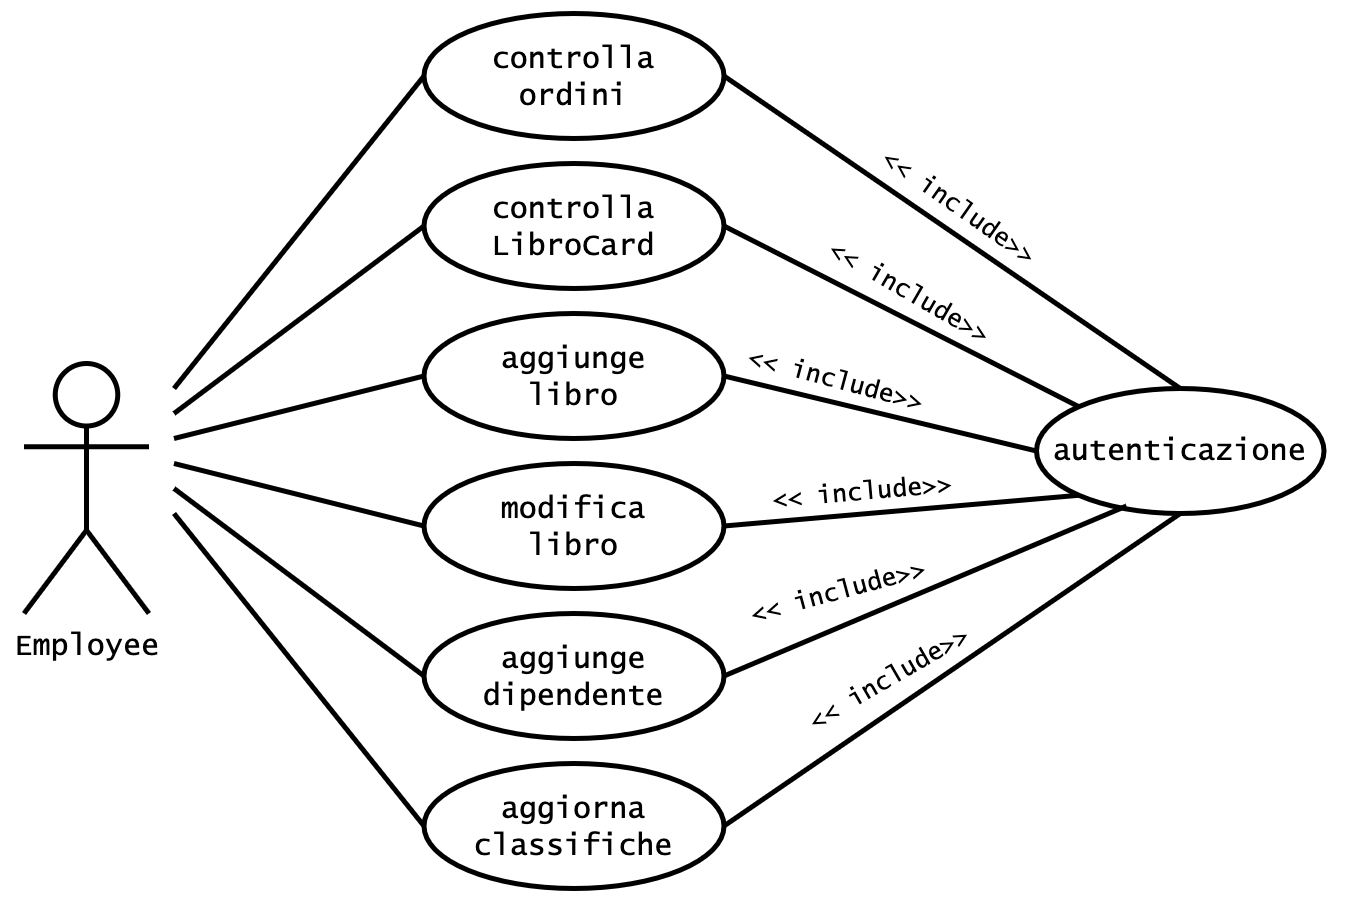
\includegraphics[scale=0.4]{images/UseCaseDiagrams/EmployeeDiagram.png}
		\caption{Use case diagram per il responsabile di libreria (employee)}
	\end{figure}
	\newpage
	\begin{figure}[h!]
		\centering
		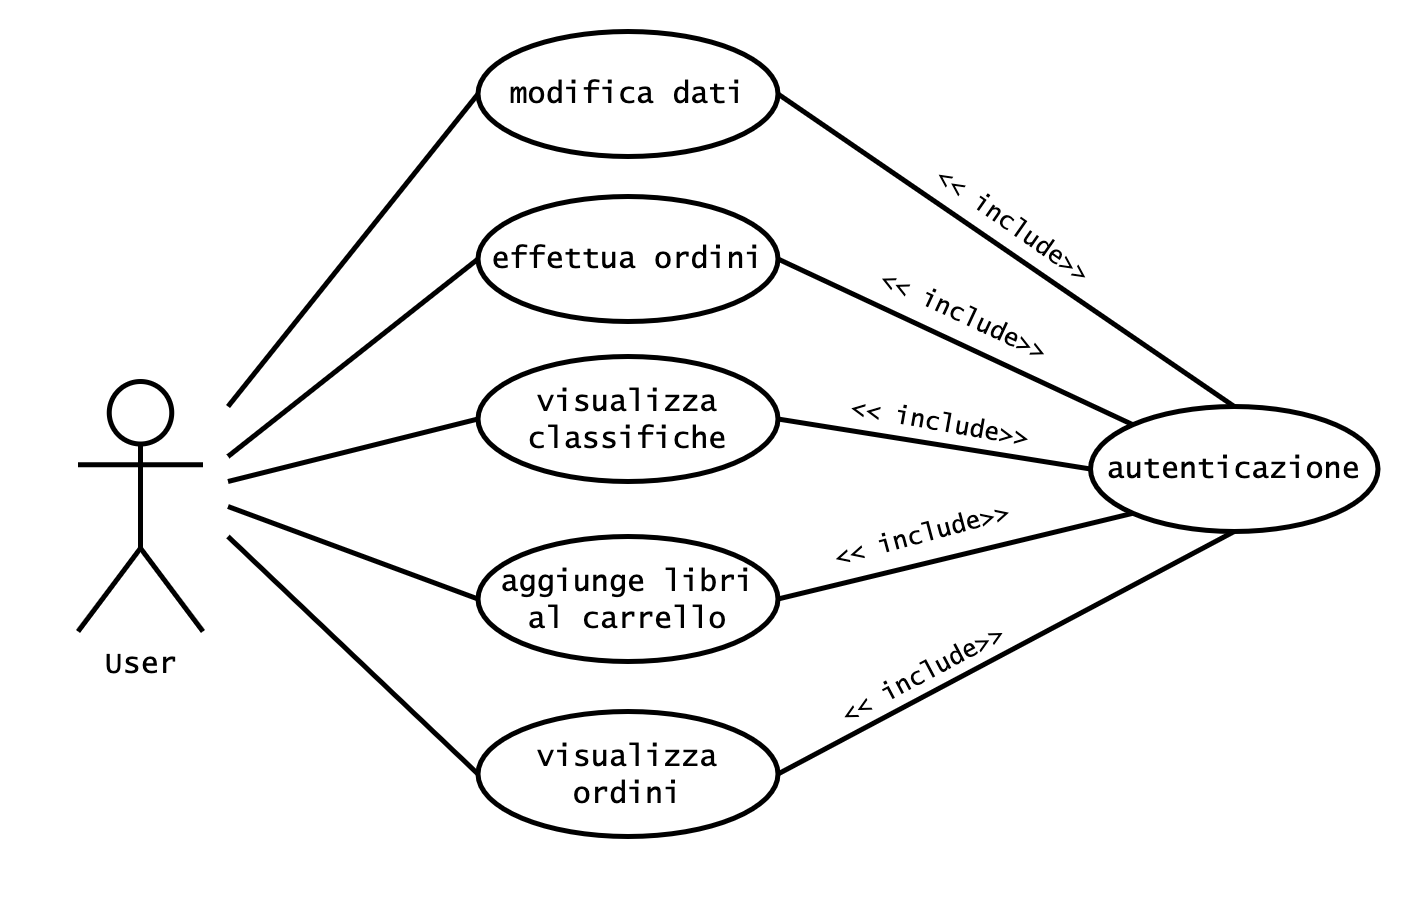
\includegraphics[scale=0.4]{images/UseCaseDiagrams/UserDiagram.png}
		\caption{Use case diagram per l'utente registrato}
	\end{figure}
	\vspace{20px}
	\begin{figure}[h!]
		\centering
		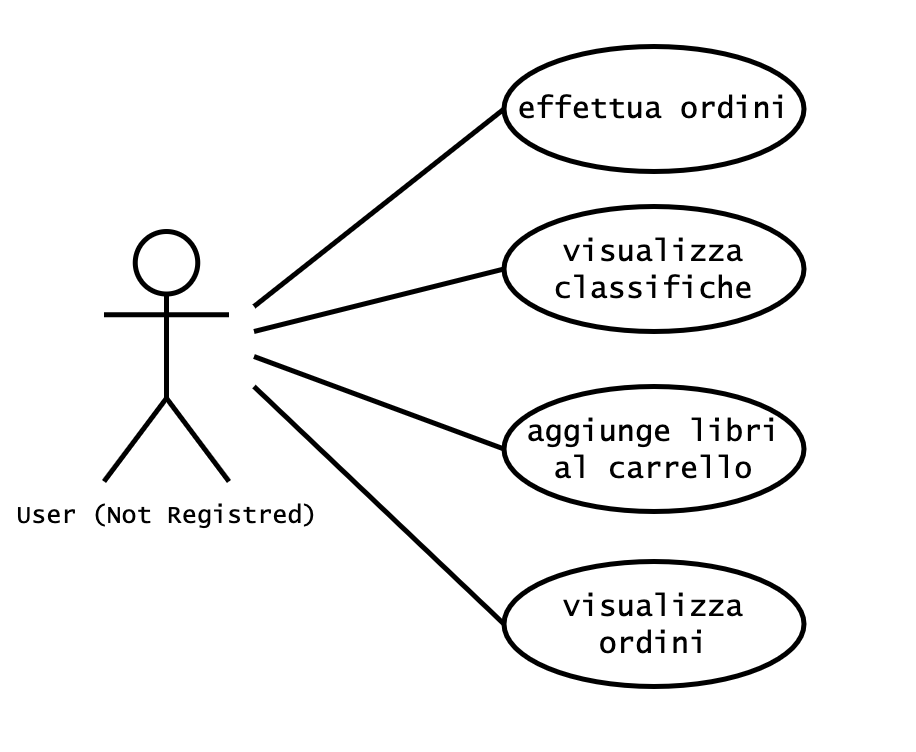
\includegraphics[scale=0.4]{images/UseCaseDiagrams/UserNotRegistredDiagram.png}
		\caption{Use case diagram per l'utente non registrato}
	\end{figure}
	% ridefinisco lo spazio tra righe
	\renewcommand{\arraystretch}{2.0}
	% aumento lo spazio tra colonne
	\setlength{\tabcolsep}{15pt}
	\newpage
	\begin{tabular}{|l|l|}
		\hline
		\textbf{ID} & UC1: Controllo ordini\\
		\hline
		\textbf{Attori} & Responsabile di libreria\\
		\hline
		\textbf{Precondizioni} & Il responsabile di libreria deve aver effettuato il log in\\
		\hline
		\textbf{Sequenza} & \makecell[l]{\\1) Dalla ChoiceBox, il responsabile filtra gli ordini in base\\
			\hspace{15px}allo stato\vspace{5px}\\
			\hspace{15px}1.2) Se non esiste alcun ordine che si trova nello stato sele-\\
			\hspace{38px}zionato, viene presentato un avviso\vspace{5px}\\}\\
		\hline
		\textbf{Postcondizione} & \makecell[l]{Viene visualizzata la LibroCard ricercata, se presente.}\\
		\hline
	\end{tabular}
	\newpage 
	\begin{tabular}{|l|l|}
		\hline
		\textbf{ID} & UC2: Controllo LibroCard\\
		\hline
		\textbf{Attori} & Responsabile di libreria\\
		\hline
		\textbf{Precondizioni} & Il responsabile di libreria deve aver effettuato il log in\\
		\hline
		\textbf{Sequenza} & \makecell[l]{\\1) Dalla \texttt{MainPage} il responsabile clicca sul pulsante \texttt{Check}\\ \hspace{15px}\texttt{LibroCards}\vspace{5px}\\
			2) Dalla pagina di controllo delle LibroCard, il responsabile\\
			\hspace{15px}può decidere come effettuare la ricerca della specifica Li-\\
			\hspace{15px}broCard:\vspace{5px}\\
			\hspace{15px}2.1) Se decide di effettuare la ricerca in base all'e-mail\\
			\hspace{38px}dell'utente:
			\vspace{5px}\\
			\hspace{38px}2.1.1) Allora seleziona il bottone \texttt{e-mail}\vspace{5px}\\
			\hspace{38px}2.1.2) Inserisce l'e-mail dell'utente nel campo appo-\\
			\hspace{72px}sito
			\vspace{5px}\\
			\hspace{38px}2.1.3 Clicca il pulsante \texttt{Search}\vspace{5px}\\
			\hspace{15px}2.2) Se decide di effettuare la ricerca in base al codice uni-\\
			\hspace{38px}voco della carta (\textit{cardID}):
			\vspace{5px}\\
			\hspace{38px}2.2.1) Allora seleziona il bottone \texttt{cardID}\vspace{5px}\\
			\hspace{38px}2.2.2) Inserisce la cardID nel campo appo-\\
			\hspace{72px}sito
			\vspace{5px}\\
			\hspace{38px}2.2.3) Clicca il pulsante \texttt{Search}\vspace{5px}\\
		}\\
		\hline
		\textbf{Caso d'eccezione} & \makecell[l]{\\Se i parametri di ricerca non corrispondono ad alcuna Libro-\\Card registrata, si presenta un messaggio d'errore\vspace{5px}\\}\\
		\hline
		\textbf{Postcondizione} & \makecell[l]{Viene visualizzata la LibroCard ricercata, se presente.}\\
		\hline
	\end{tabular}
	\newpage 
	\begin{tabular}{|l|l|}
		\hline
		\textbf{ID} & UC3: Inserimento di un nuovo libro\\
		\hline
		\textbf{Attori} & Responsabile di libreria\\
		\hline
		\textbf{Precondizioni} & Il responsabile di libreria deve aver effettuato il log in\\
		\hline
		\textbf{Sequenza} & \makecell[l]{\\1) Dalla \texttt{MainPage} il responsabile clicca sul pulsante \texttt{Add a}\\ \hspace{15px}\texttt{new book}\vspace{5px}\\
			2) Il responsabile inserisce tutti i dati richiesti negli appositi\\
			\hspace{15px}campi
			\vspace{5px}\\
			3) Il responsabile clicca sul pulsante \texttt{Add book}\vspace{5px}\\
			4) Si apre un messaggio che informa la corretta aggiunta del \\
			\hspace{15px}libro\vspace{5px}\\}\\
		\hline
		\textbf{Caso d'eccezione} & \makecell[l]{\\1) Se il responsabile non inserisce tutti i dati richiesti, viene\\
			\hspace{15px}presentato un messaggio d'errore e l'inserimento del libro\\
			\hspace{15px}viene bloccato\vspace{5px}\\
			2) Se l'ISBN specificato corrisponde a quello di un libro già\\
			\hspace{15px} registrato nel database, viene presentato un messaggio\\
			\hspace{15px}d'errore e l'inserimento del libro viene bloccato\vspace{5px}\\}\\ 
		\hline
		\textbf{Postcondizione} & \makecell[l]{Viene visualizzata la LibroCard ricercata, se presente.}\\
		\hline
	\end{tabular}
	\newpage 
	\begin{tabular}{|l|l|}
		\hline
		\textbf{ID} & UC4: Modifica di un libro\\
		\hline
		\textbf{Attori} & Responsabile di libreria\\
		\hline
		\textbf{Precondizioni} & Il responsabile di libreria deve aver effettuato il log in\\
		\hline
		\textbf{Sequenza} & \makecell[l]{\\1) Dalla \texttt{MainPage} il responsabile clicca sul pulsante \texttt{Modify}\\ \hspace{15px}\texttt{books}\vspace{5px}\\
			2) Il responsabile inserisce l'ISBN del libro da modificare
			\vspace{5px}\\
			3) Il responsabile inserisce solo i campi che desidera modificare\vspace{5px}\\
			4) Se il responsabile clicca sul pulsante \texttt{Confirm changes}\vspace{5px}\\}\\
		\hline
		\textbf{Caso d'eccezione} & \makecell[l]{\\Se l'ISBN non corrisponde a un libro registrato, viene presenta-\\
		to un messaggio d'errore\vspace{5px}}\\
		\hline
		\textbf{Postcondizione} & \makecell[l]{Viene visualizzata la LibroCard ricercata, se presente.}\\
		\hline
	\end{tabular}	
	\newpage
	\begin{tabular}{|l|l|}
		\hline
		\textbf{ID} & UC5: Inserimento di un nuovo dipendente\\
		\hline
		\textbf{Attori} & Responsabile di libreria\\
		\hline
		\textbf{Precondizioni} & \makecell[l]{\\1) Il responsabile di libreria deve aver effettuato il log in\vspace{5px}\\
			2) Il responsabile deve avere ruolo di \texttt{General Director} \\
			\hspace{15px}oppure \texttt{Local Director}\vspace{5px}}\\
		\hline
		\textbf{Sequenza} & \makecell[l]{\\1) Dalla \texttt{MainPage}, il responsabile clicca sul pulsante \texttt{Add}\\
			\hspace{15px}\texttt{a new Employee}\vspace{5px}\\
			2) Il responsabile inserisce tutti i dati richiesti relativi al\\
			\hspace{15px}nuovo dipendente negli appositi campi 
			\vspace{5px}\\
			3) Il responsabile clicca sul pulsante \texttt{Register}\vspace{5px}\\
			4) Se i dati inseriti sono tutti validi, si apre un messaggio\\
			\hspace{15px}che informa la corretta aggiunta del nuovo dipendente\\
			\hspace{15px}nel database\vspace{5px}\\}\\
		\hline
		\textbf{Caso d'eccezione} & \makecell[l]{\\1) Se il responsabile non ha il ruolo di \texttt{General Director} o \\
			\hspace{15px}\texttt{Local Director}, viene presentato un messaggio d'errore\\
			\hspace{15px}e l'accesso alla funzione viene negato\vspace{5px}\\
			2) Se il responsabile non ha riempito tutti i campi richiesti, \\
			\hspace{15px}viene presentato un messaggio d'errore e l'inserimento non\\
			\hspace{15px}viene effettuato\vspace{5px}\\}\\
		\hline
		\textbf{Postcondizione} & \makecell[l]{Il nuovo dipendente viene aggiunto al database.}\\
		\hline
	\end{tabular}
	\newpage 
	\begin{tabular}{|l|l|}
		\hline
		\textbf{ID} & UC6: Aggiornamento classifiche\\
		\hline
		\textbf{Attori} & Responsabile di libreria\\
		\hline
		\textbf{Precondizioni} & \makecell[l]{Il responsabile di libreria deve aver effettuato il log in\vspace{5px}}\\
		\hline
		\textbf{Sequenza} & \makecell[l]{\\1) Dalla \texttt{MainPage}, il responsabile di libreria clicca il \\
		\hspace{15px}pulsante \texttt{Update Rankings}\vspace{5px}\\
		2) Dalla pagina di aggiornamento classifiche, il respon-\\
		\hspace{15px}sabile clicca il pulsante \texttt{Update} \vspace{5px}\\}\\
		\hline
		\textbf{Postcondizione} & \makecell[l]{Le classifiche sono state aggiornate}\\
		\hline
	\end{tabular}
	\newpage
	\begin{tabular}{|l|l|}
		\hline
		\textbf{ID} & UC7: Modifica dei dati personali\\
		\hline
		\textbf{Attori} & Utente registrato\\
		\hline
		\textbf{Precondizioni} & \makecell[l]{L'utente deve aver effettuato il log in\vspace{5px}\\}\\
		\hline
		\textbf{Sequenza} & \makecell[l]{\\1) Dalla pagina del profilo, l'utente clicca il pulsante \texttt{Modify} \\ \texttt{your data}, che porta alla pagina di modifica dei dati\vspace{5px}\\
			2) L'utente riempie esclusivamente i campi che desidera modifi-\\care\vspace{5px}\\
			3) Se l'utente clicca sul pulsante \texttt{Confirm changes}, si apre un \\messaggio che richiede la conferma della modifica:\vspace{5px}\\
			\hspace{11px} 3.1) Se l'utente clicca sul pulsante \texttt{OK} del dialog, i dati nel\\ 
			\hspace{38px}database vengono modificati e l'utente viene riportato \\
			\hspace{38px}nella pagina del profilo\vspace{5px}\\
			\hspace{11px} 3.2) Se l'utente clicca sul pulsante \texttt{Cancel}, il dialog si chiude\\
			\hspace{38px}e si resta nella pagina di modifica dei dati\vspace{5px}\\
			4) Se l'utente clicca sul pulsante \texttt{Cancel} della pagina, si apre un\\
			messaggio che richiede la conferma dell'azione:\vspace{5px}\\
			\hspace{11px} 4.1) Se l'utente clicca il pulsante \texttt{OK} del dialog, si viene ripor-\\
			\hspace{38px}tati nella pagina del profilo e i dati restano immutati\vspace{5px}\\
			\hspace{11px} 4.2) Se l'utente clicca il pulsante \texttt{Cancel} del dialog, si resta \\
			\hspace{38px} nella pagina di modifica dei dati\vspace{5px}}\\
		\hline
		\textbf{Postcondizioni} & I dati dell'utente vengono modificati\\
		\hline
	\end{tabular}
	\newpage
	\begin{tabular}{|l|l|}
		\hline
		\textbf{ID} & UC8: Creazione di un ordine\\
		\hline
		\textbf{Attori} & Utente registrato\\
		\hline
		\textbf{Precondizioni} & \makecell[l]{\\1. L'utente deve aver effettuato il log in\vspace{5px}\\2. Il carrello dell'utente deve avere almeno un articolo\vspace{5px}\\}\\
		\hline
		\textbf{Sequenza} & \makecell[l]{\\1) Dalla pagina del carrello, l'utente clicca il pulsante \texttt{Check Out}\vspace{5px}\\
		2) L'utente seleziona un metodo di pagamento\vspace{5px}\\
		3) L'utente sceglie l'indirizzo di spedizione, che può essere quello \\di domicilio o un altro indirizzo \vspace{5px}\\
		\hspace{15px} 3.a) Se l'utente sceglie un indirizzo diverso da quello del domi-\\\hspace{15px}cilio, allora deve specificare l'indirizzo nel campo apposito\vspace{5px}\\
		4) L'utente clicca sul pulsante \texttt{Check Out}\vspace{5px}\\}\\
		\hline
		\textbf{Caso d'eccezione} & \makecell[l]{\\1) Se il carrello è vuoto, viene presentato un messaggio d'errore\\
		\hspace{15px}che impedisce di procedere all'acquisto\vspace{5px}\\
		2) Se l'utente non ha selezionato un metodo di pagamento o non\\
		\hspace{15px}ha specificato l'indirizzo alternativo, viene presentato un mes-\\\hspace{15px}saggio di errore che richiede l'inserimento dei dati mancanti\vspace{5px}\\}\\
		\hline
		\textbf{Postcondizioni} & L'ordine viene confermato\\
		\hline
	\end{tabular}
	\newpage
	\begin{tabular}{|l|l|}
		\hline
		\textbf{ID} & UC9: Visualizzazione classifiche\\
		\hline
		\textbf{Attori} & Utente generico\\
		\hline
		\textbf{Precondizioni} & \\
		\hline
		\textbf{Sequenza} & \makecell[l]{\\1) Dalla \texttt{MainPage}, l'utente clicca il pulsante \texttt{Rankings}\vspace{5px}\\
		2) Dalla pagina delle classifiche, l'utente può selezionare\\
		\hspace{15px} un genere di cui visualizzare la relativa classifica \vspace{5px}\\}\\
		\hline
		\textbf{Postcondizione} & \\
		\hline
	\end{tabular}\vspace{35px}\\
	\begin{tabular}{|l|l|}
		\hline
		\textbf{ID} & UC10: Aggiunta di un libro al carrello\\
		\hline
		\textbf{Attori} & Utente generico\\
		\hline
		\textbf{Precondizioni} & \\
		\hline
		\textbf{Sequenza} & \makecell[l]{\\1) Dalla \texttt{MainPage}, l'utente seleziona un libro\vspace{5px}\\
			2) L'utente viene portato nella pagina contenente tutte le infor-\\
			\hspace{15px}mazioni relative al libro\vspace{5px}\\
			3) Se l'utente desidera più di una copia di quel libro, può sele-\\
			\hspace{15px}zionare fino a dieci unità tramite lo Spinner a destra\vspace{5px}\\
			4) L'utente clicca sul pulsante \texttt{Add To Cart} per aggiungere il \\
			\hspace{15px}libro\vspace{5px}\\}\\
		\hline
		\textbf{Caso d'eccezione} & \makecell[l]{\\1) Se non ci sono più copie di quel libro, viene presentato un \\
			\hspace{15px}messaggio d'errore e il libro non viene aggiunto\vspace{5px}\\
			2) Se il libro è già presente nel carrello, viene presentato un\\
			\hspace{15px}messaggio di errore e il libro non viene aggiunto\vspace{5px}\\}\\
		\hline
		\textbf{Postcondizione} & \makecell[l]{Il libro è stato aggiunto al carrello}\\
		\hline
	\end{tabular}
	\newpage 
	\begin{tabular}{|l|l|}
		\hline
		\textbf{ID} & UC11: Visualizzazione ordini\\
		\hline
		\textbf{Attori} & Utente registrato\\
		\hline
		\textbf{Precondizioni} & \makecell[l]{\\L'utente deve essere registrato\vspace{5px}\\}\\
		\hline
		\textbf{Sequenza} & \makecell[l]{\\1) Se l'utente si trova nella \texttt{MainPage}, clicca sulla scritta \texttt{MY}\\ \hspace{15px}\texttt{ORDERS}\vspace{5px}\\
		2) Se l'utente si trova sulla pagina del profilo, clicca sul pul-\\
		\hspace{15px}sante \texttt{MY ORDERS}\vspace{5px}\\}\\
		\hline
		\textbf{Postcondizioni} & \\
		\hline
	\end{tabular}
	\vspace{35px}\\
	\begin{tabular}{|l|l|}
		\hline
		\textbf{ID} & UC12: Ricerca di un ordine\\
		\hline
		\textbf{Attori} & Utente generico\\
		\hline
		\textbf{Precondizioni} & L'utente non deve aver effettuato il log in\\
		\hline
		\textbf{Sequenza} & \makecell[l]{\\1) Dalla \texttt{MainPage}, l'utente clicca sulla scritta \texttt{MY ORDERS}\vspace{5px}\\
		2) L'utente inserisce il codice dell'ordine nel campo apposito\vspace{5px}\\
		3) L'utente clicca sul pulsante \texttt{Search}\vspace{5px}\\}\\
		\hline
		\textbf{Caso d'eccezione} & \makecell[l]{\\Se il codice inserito non corrisponde ad alcun ordine registra-\\ 
		to, viene presentato un messaggio di errore\vspace{5px}}\\
		\hline
		\textbf{Postcondizioni} & \makecell[l]{\\L'utente visualizza le informazioni relative al suo ordine, se \\questo è presente\vspace{5px}\\}\\
		\hline
	\end{tabular}
	\newpage
	\begin{tabular}{|l|l|}
		\hline
		\textbf{ID} & UC13: Creazione di un ordine\\
		\hline
		\textbf{Attori} & Utente non registrato\\
		\hline
		\textbf{Precondizioni} & \makecell[l]{Il carrello dell'utente deve avere almeno un articolo\vspace{5px}\\}\\
		\hline
		\textbf{Sequenza} & \makecell[l]{\\1) Dalla pagina del carrello, l'utente clicca il pulsante \texttt{Check Out}\vspace{5px}\\
		2) L'utente deve specificare: nome, cognome, metodo di pagamen-\\
		\hspace{15px}to, un indirizzo di spedizione e le informazioni di contatto nei\\
		\hspace{15px}campi appositi \vspace{5px}\\
		3) L'utente clicca sul pulsante \texttt{Check Out}\vspace{5px}\\}\\
		\hline
		\textbf{Caso d'eccezione} & \makecell[l]{\\1) Se il carrello è vuoto, viene presentato un messaggio d'errore\\
		\hspace{15px}che impedisce di procedere all'acquisto\vspace{5px}\\
		2) Se l'utente non ha inserito tutti i campi richiesti, viene presen-\\\hspace{15px}tato un messaggio d'errore che impedisce di completare\\\hspace{15px} l'acquisto\vspace{5px}\\}\\
		\hline
		\textbf{Postcondizioni} & L'ordine viene confermato\\
		\hline
	\end{tabular}
	\vspace{20px}
	\begin{tabular}{|l|l|}
		\hline
		\textbf{ID} & UC15: Ricerca di un ordine\\
		\hline
		\textbf{Attori} & Utente non registrato\\
		\hline
		\textbf{Precondizioni} & \\
		\hline
		\textbf{Sequenza} & \makecell[l]{\\1) Dalla \texttt{MainPage}, l'utente clicca sulla scritta \texttt{MY ORDERS} in\\alto
		a sinistra\vspace{5px}\\
		2) L'utente viene portato nella pagina di relativa al traccia-\\mento degli ordini\vspace{5px}\\
		3) L'utente inserisce nel campo apposito il codice univoco \\dell'ordine che desidera visualizzare\vspace{5px}\\
		4) L'utente clicca sul pulsante di ricerca \texttt{Search}\vspace{5px}\\}\\
		\hline
		\textbf{Caso d'eccezione} & \makecell[l]{\\Se il codice non corrisponde ad alcun ordine presente nel data-\\base, si apre un messaggio d'errore\vspace{5px}}\\
		\hline
		\textbf{Postcondizione} & \makecell[l]{\\L'utente visualizza le informazioni relative all'ordine se questo\\ è presente nel database.\vspace{5px}\\}\\
		\hline
	\end{tabular}
	\newpage
	\subsection{Activity Diagram}
	Di seguito si riportano gli activity diagrams delle operazioni principali messe a disposizione dal programma. I diagrammi  rappresentano il flusso di esecuzione che porta al compimento di una determinata funzione.\\
	\begin{figure}[h!]
		\centering
		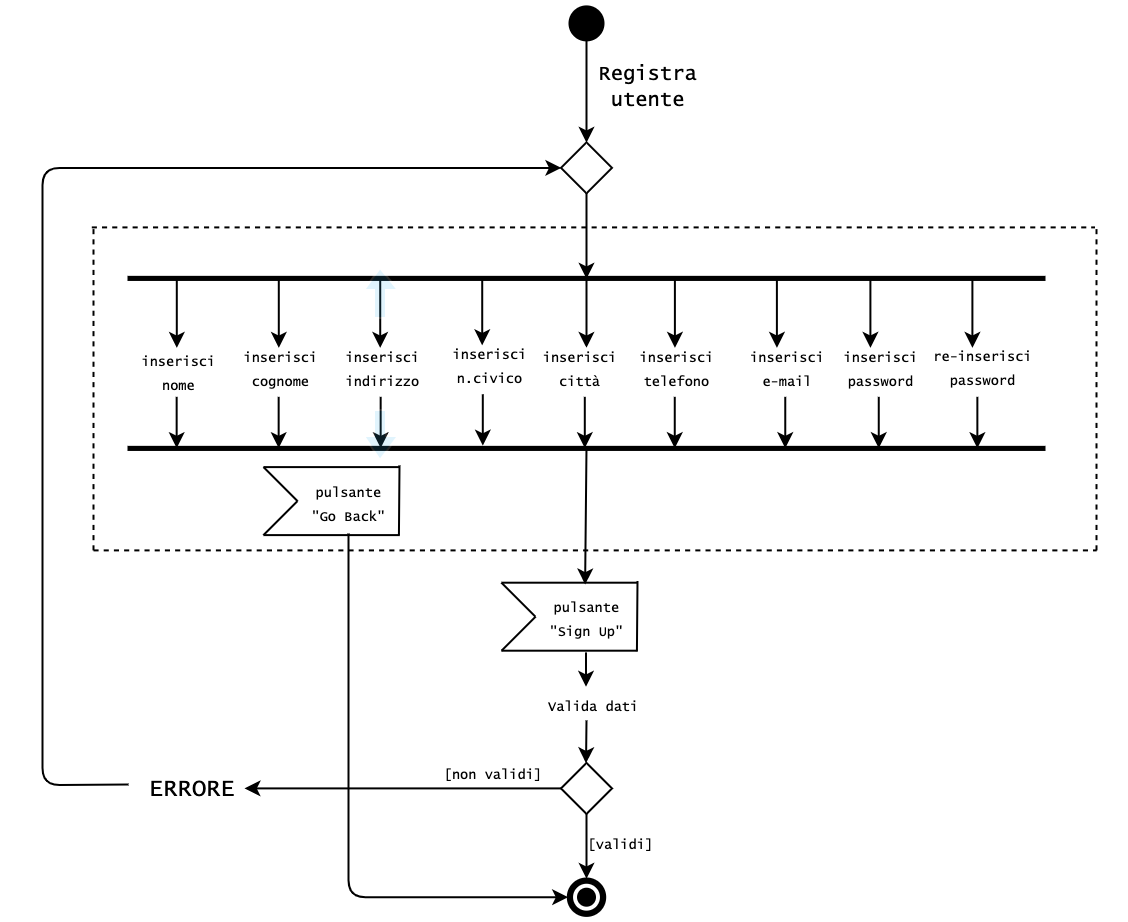
\includegraphics[scale=0.40]{images/ActivityDiagrams/RegistraUtente.png}
		\caption{Activity diagram per la \textbf{registrazione di un utente}}
	\end{figure}
	\begin{figure}[h!]
		\centering
		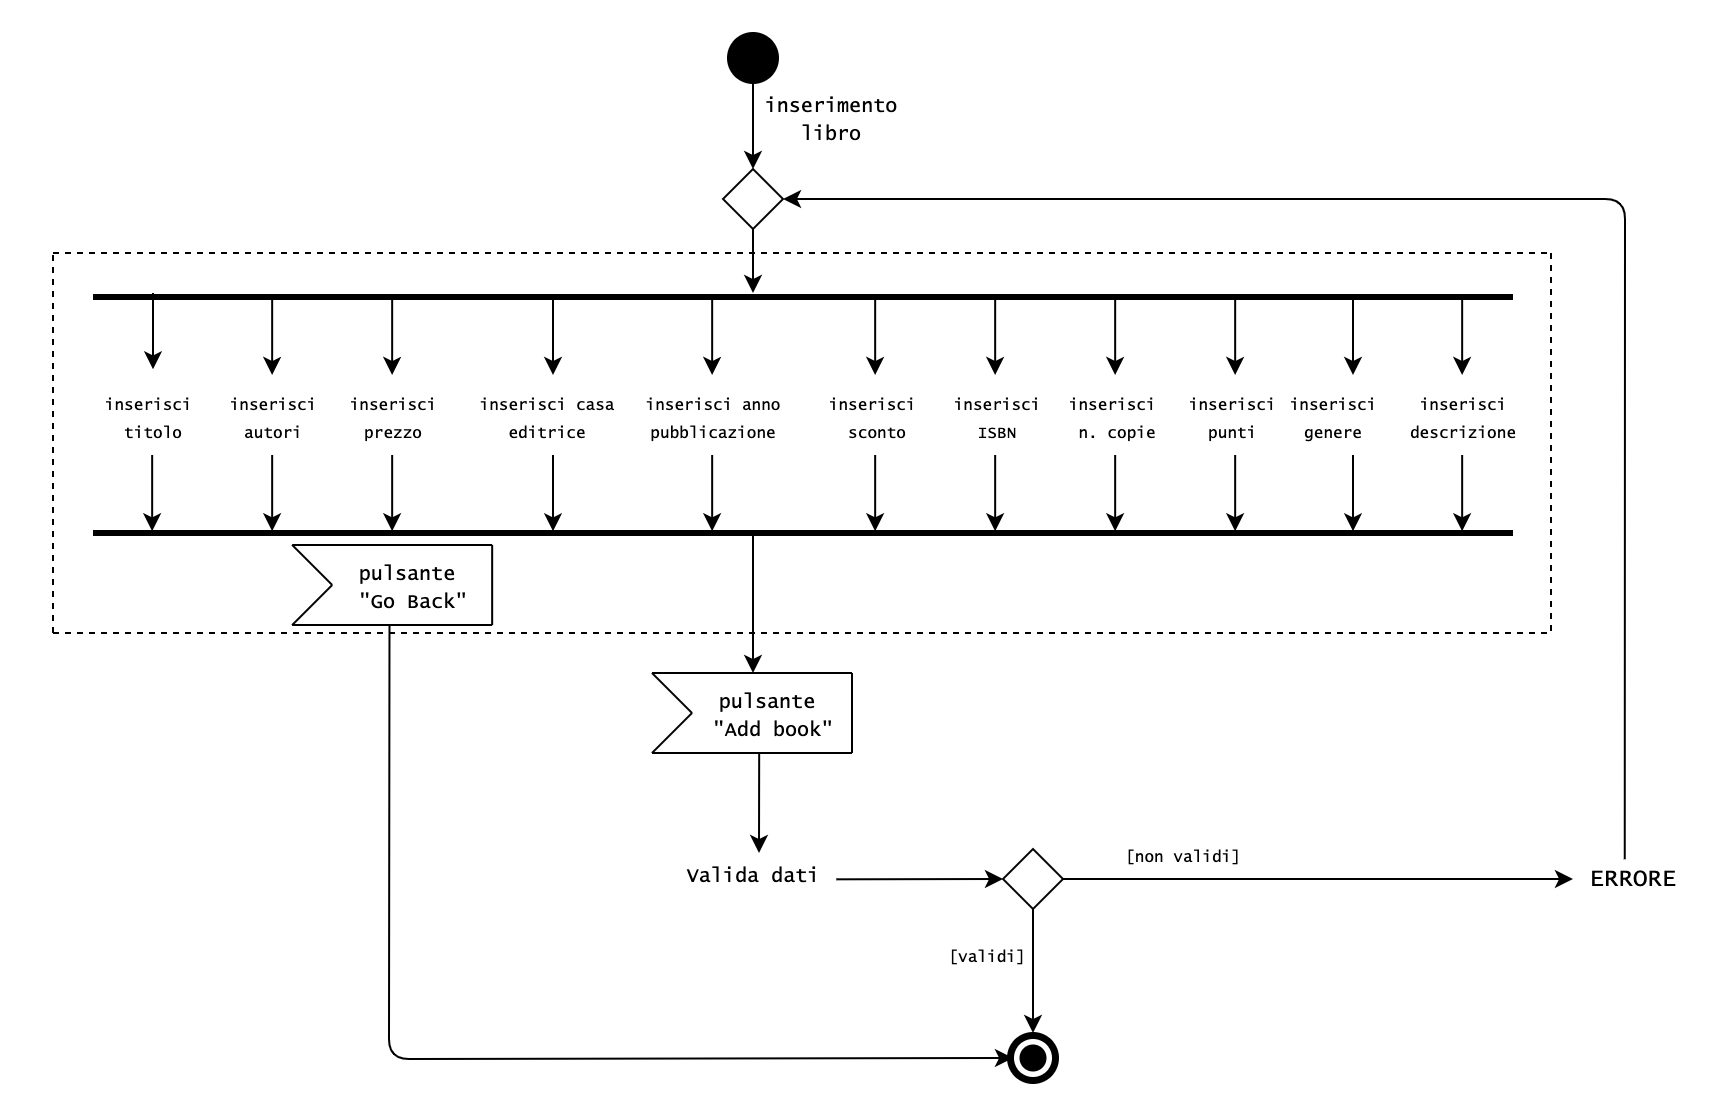
\includegraphics[scale=0.4]{images/ActivityDiagrams/InserimentoLibro.png}
		\caption{Activity diagram per l'\textbf{inserimento di un libro}}
	\end{figure}
	\newpage
	\begin{figure}[h!]
		\centering
		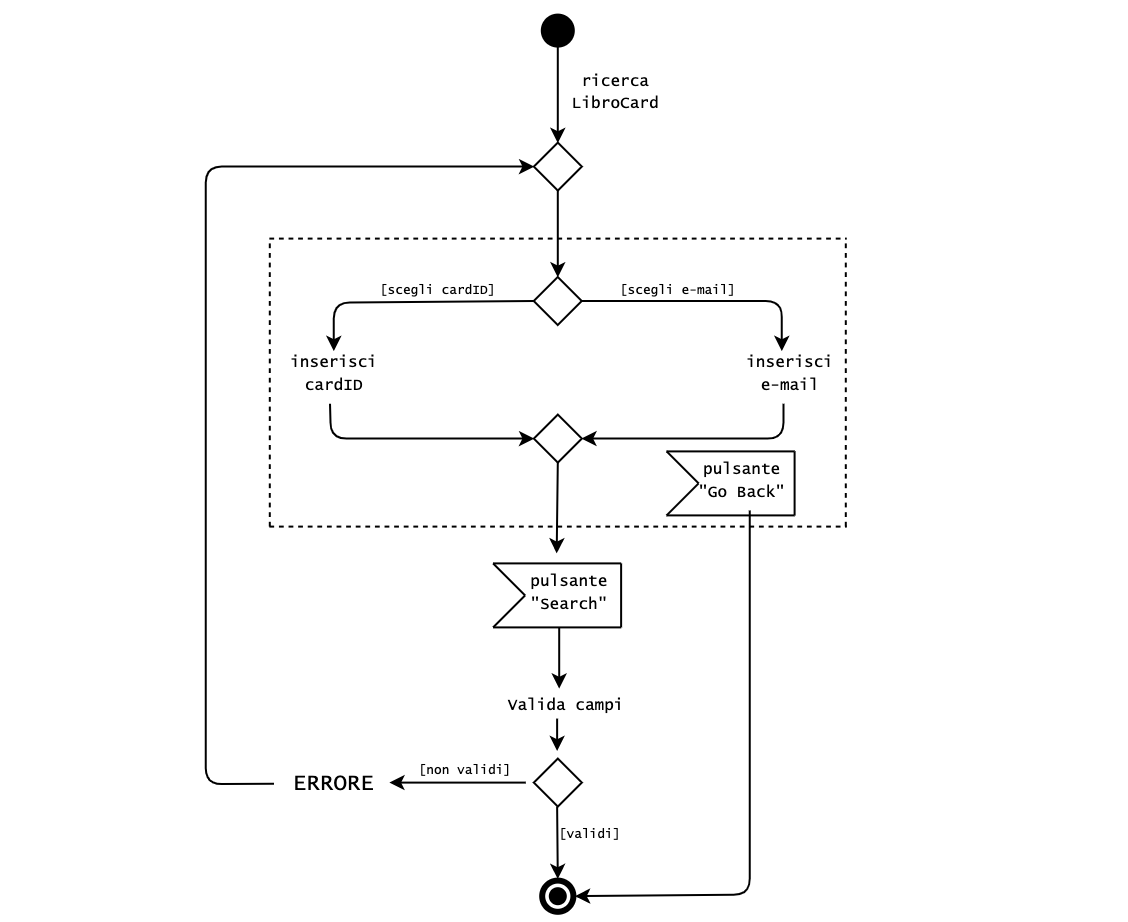
\includegraphics[scale=0.45]{images/ActivityDiagrams/RicercaLibroCard.png}
		\caption{Activity diagram per la \textbf{ricerca di una LibroCard}}
	\end{figure}
	\begin{figure}[h!]
		\centering
		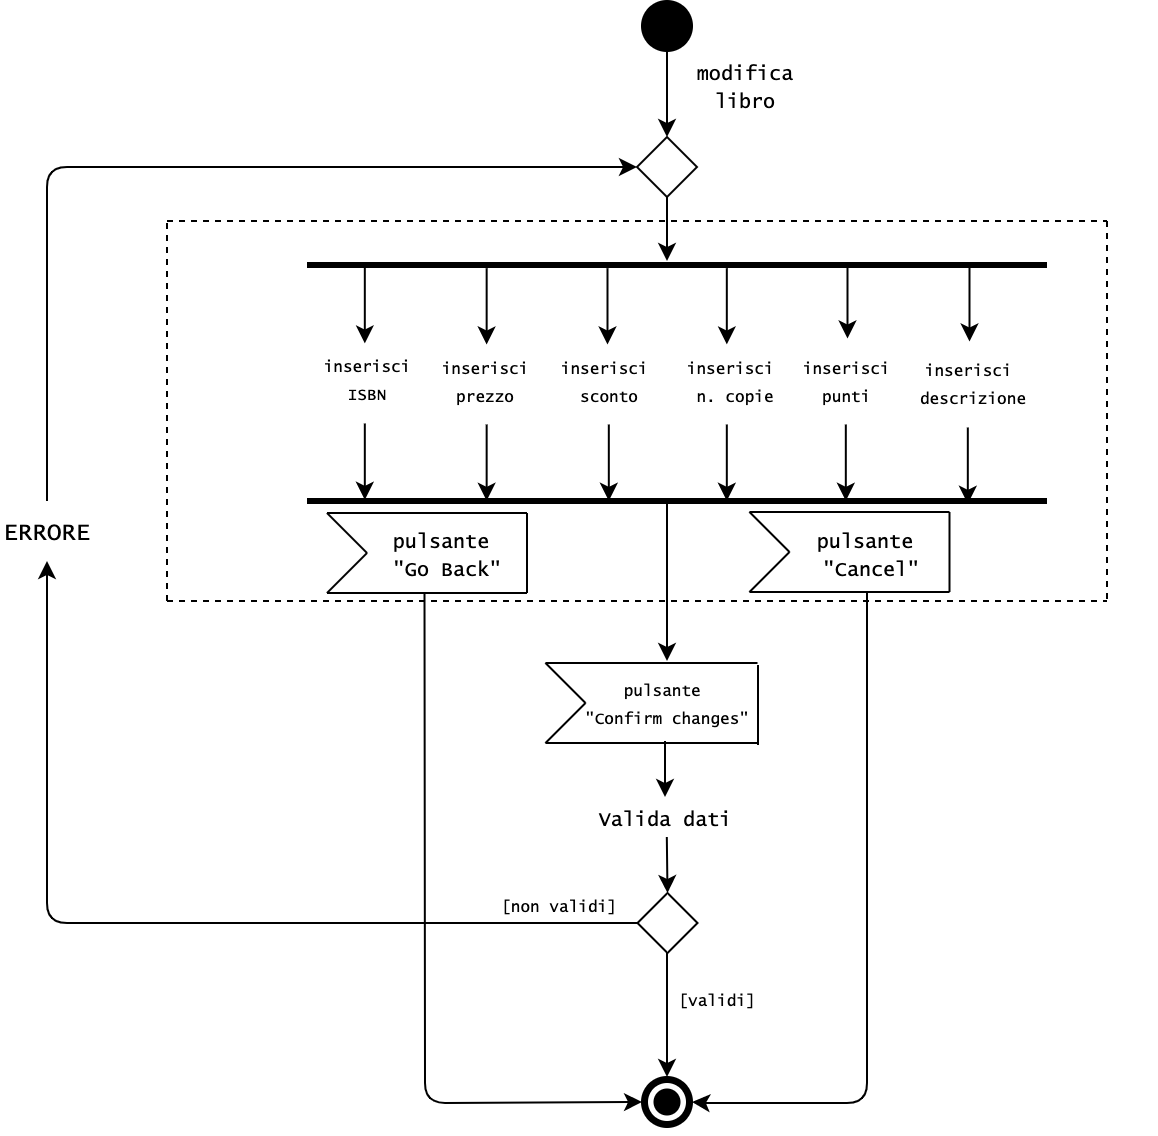
\includegraphics[scale=0.45]{images/ActivityDiagrams/ModificaLibro.png}
		\caption{Activity diagram per la \textbf{modifica di un libro}}
	\end{figure}
	\newpage
	\begin{figure}[h!]
		\centering
		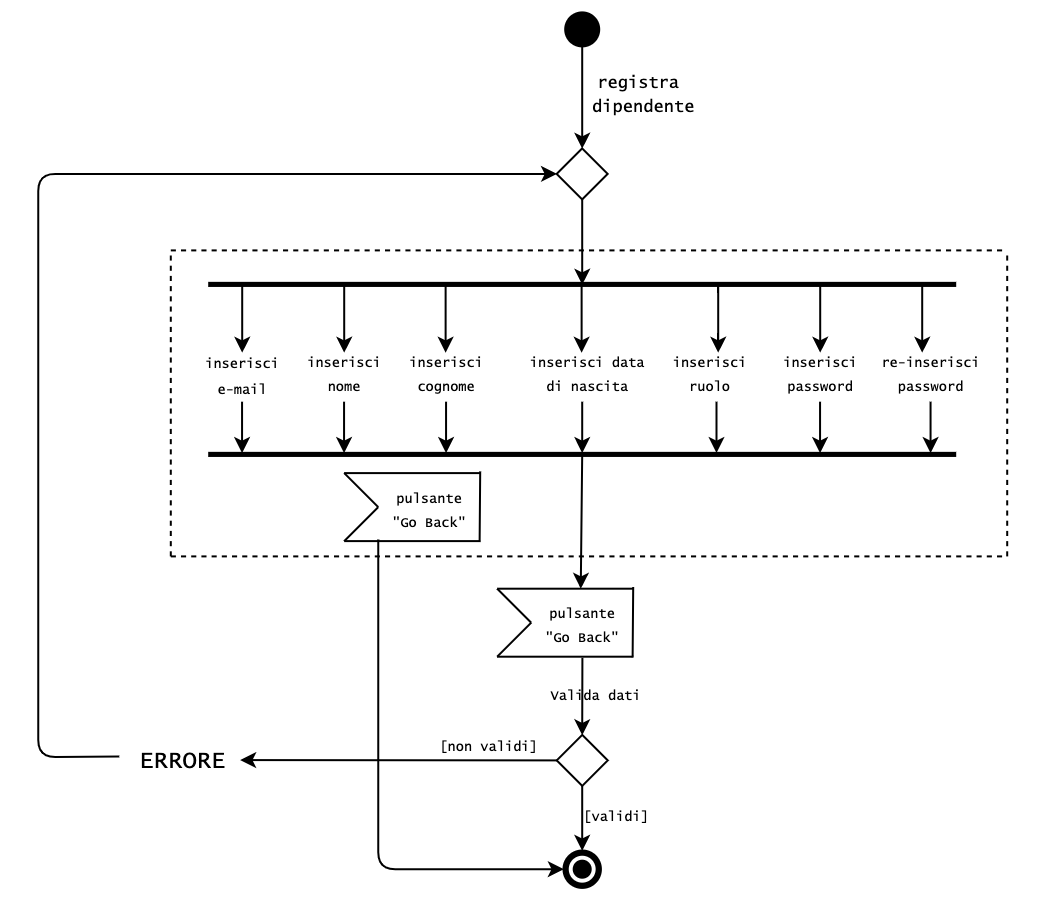
\includegraphics[scale=0.5]{images/ActivityDiagrams/RegistraDipendente.png}
		\caption{Activity diagram per l'\textbf{inserimento di un nuovo dipendente}}
	\end{figure}
	\begin{figure}[h!]
		\centering
		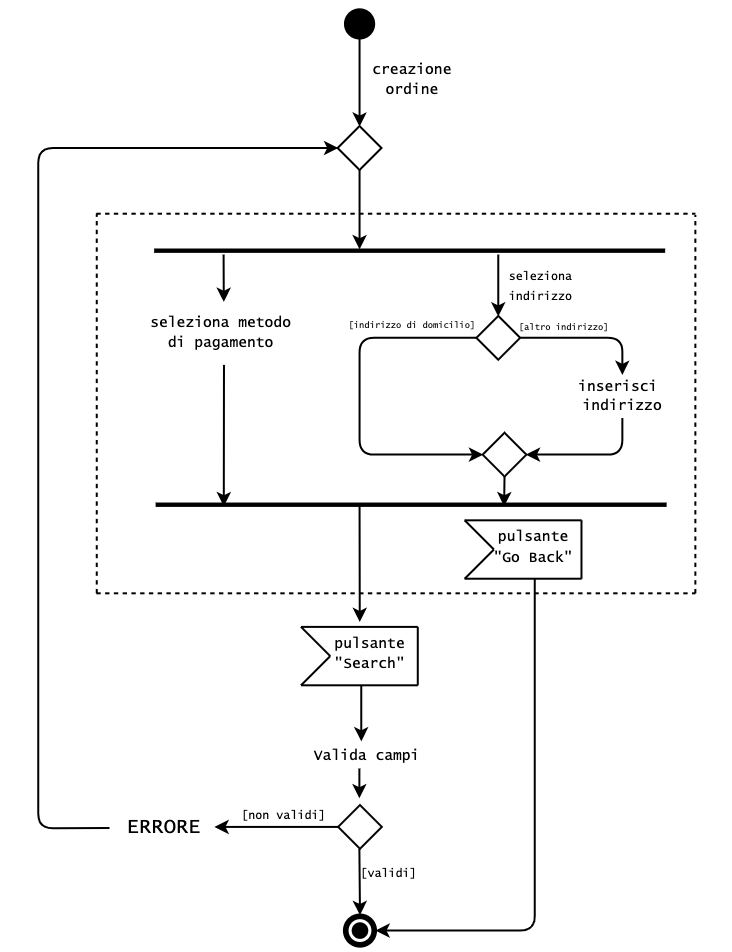
\includegraphics[scale=0.55]{images/ActivityDiagrams/CreazioneOrdineUtente.png}
		\caption{Activity diagram per la\textbf{creazione di un ordine} (utente)}
	\end{figure}
	\newpage
	\begin{figure}[h!]
		\centering
		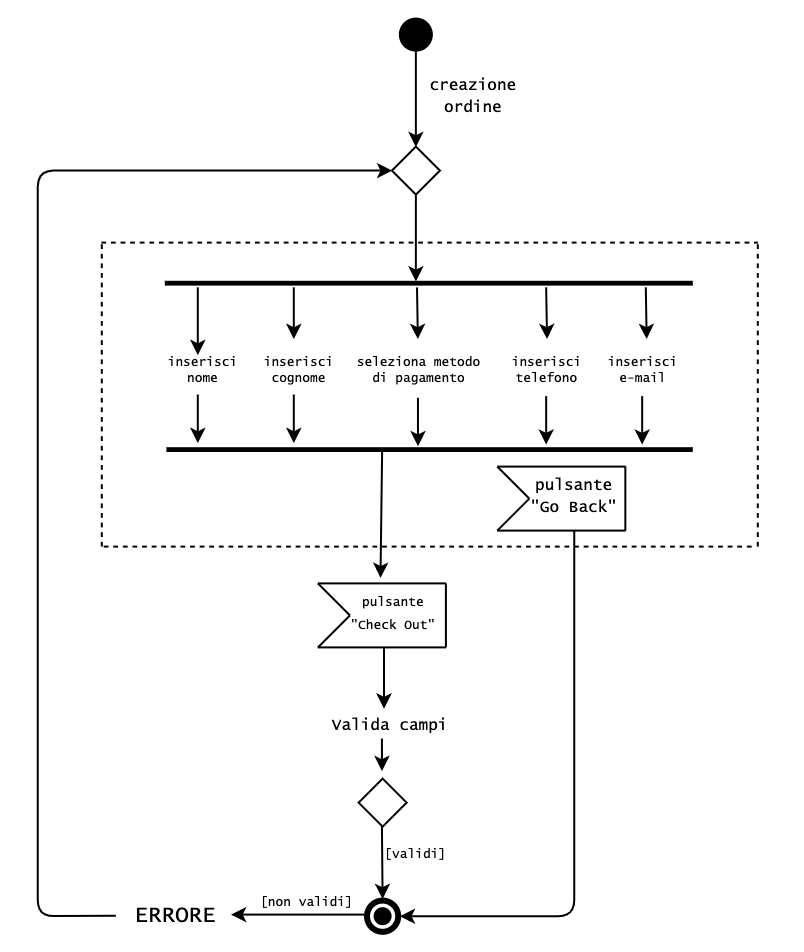
\includegraphics[scale=0.5]{images/ActivityDiagrams/CreazioneOrdineUtenteNonReg.png}
		\caption{Activity diagram per la \textbf{creazione di un ordine} (utente non registrato)}
	\end{figure}
	\newpage
	\subsection{Class Diagrams}
	In questa sezione si riportano i class diagrams, che rappresentano l'architettura del programma e aiutano a comprendere chiaramente come le varie classi interagiscono tra loro.\\
	\begin{figure}[h!]
		\centering
		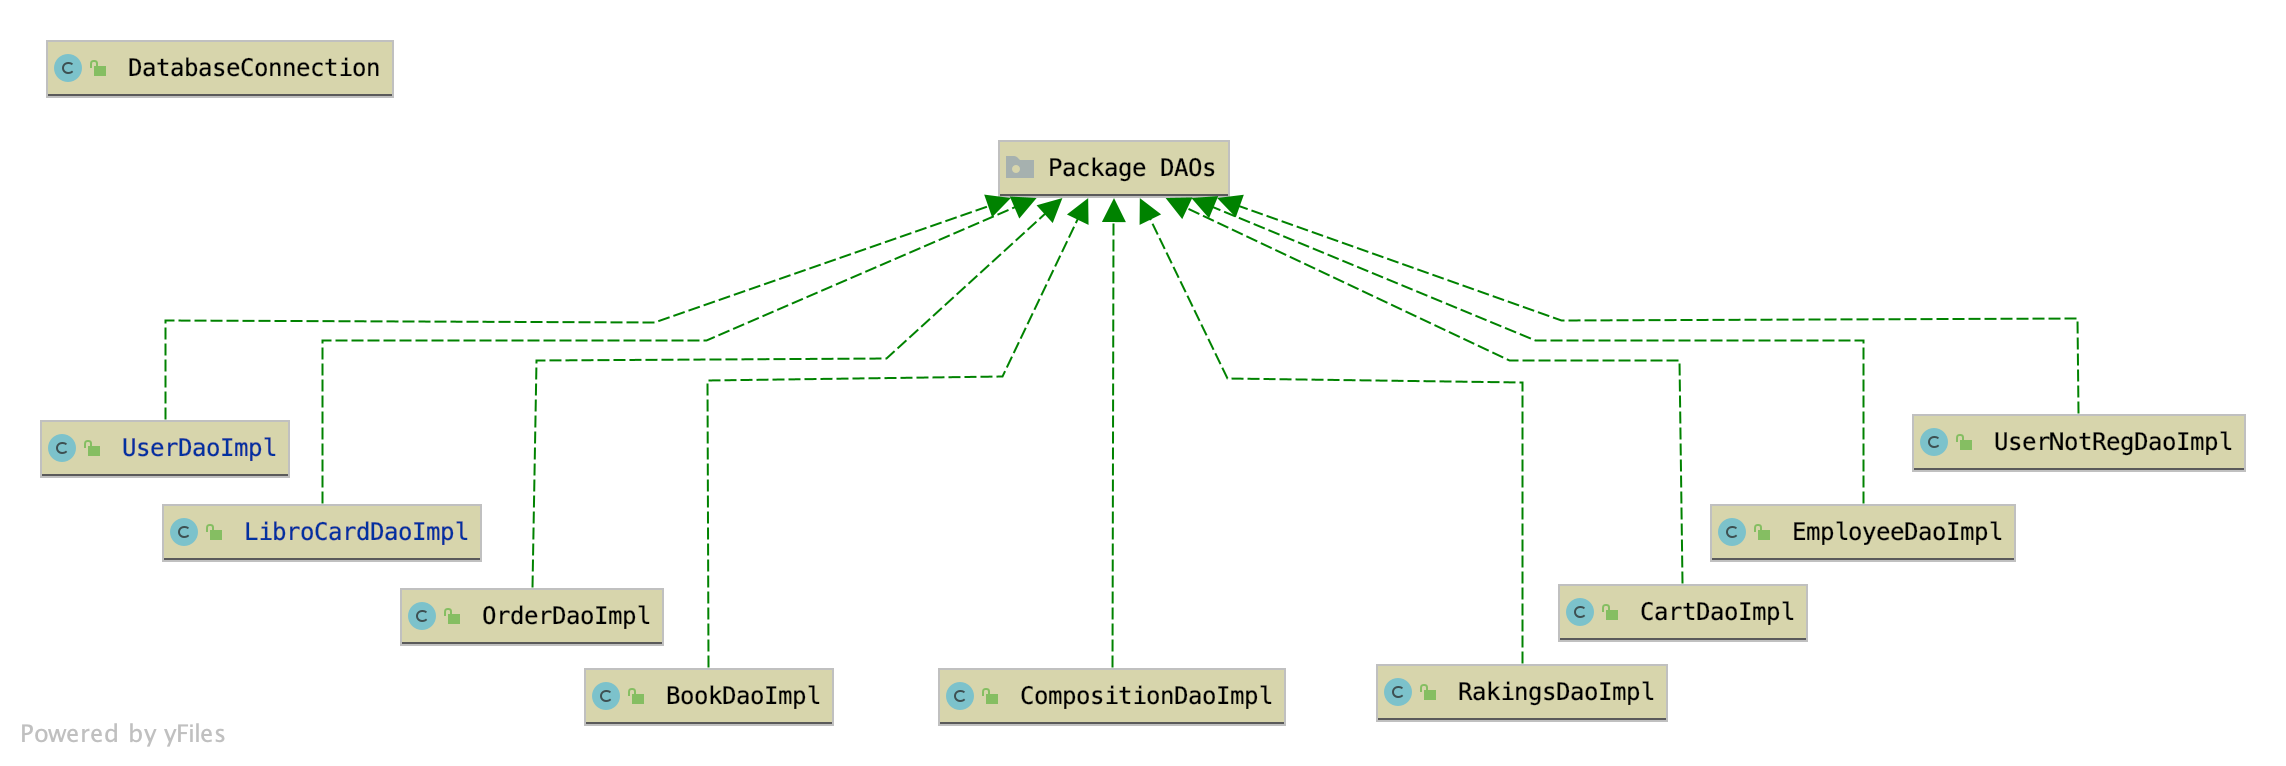
\includegraphics[scale=0.2]{images/ClassDiagrams/UtilsClassDiagram.png}
		\caption{Class Diagram per il package Utils}
	\end{figure}
	\begin{figure}[h!]
		\centering
		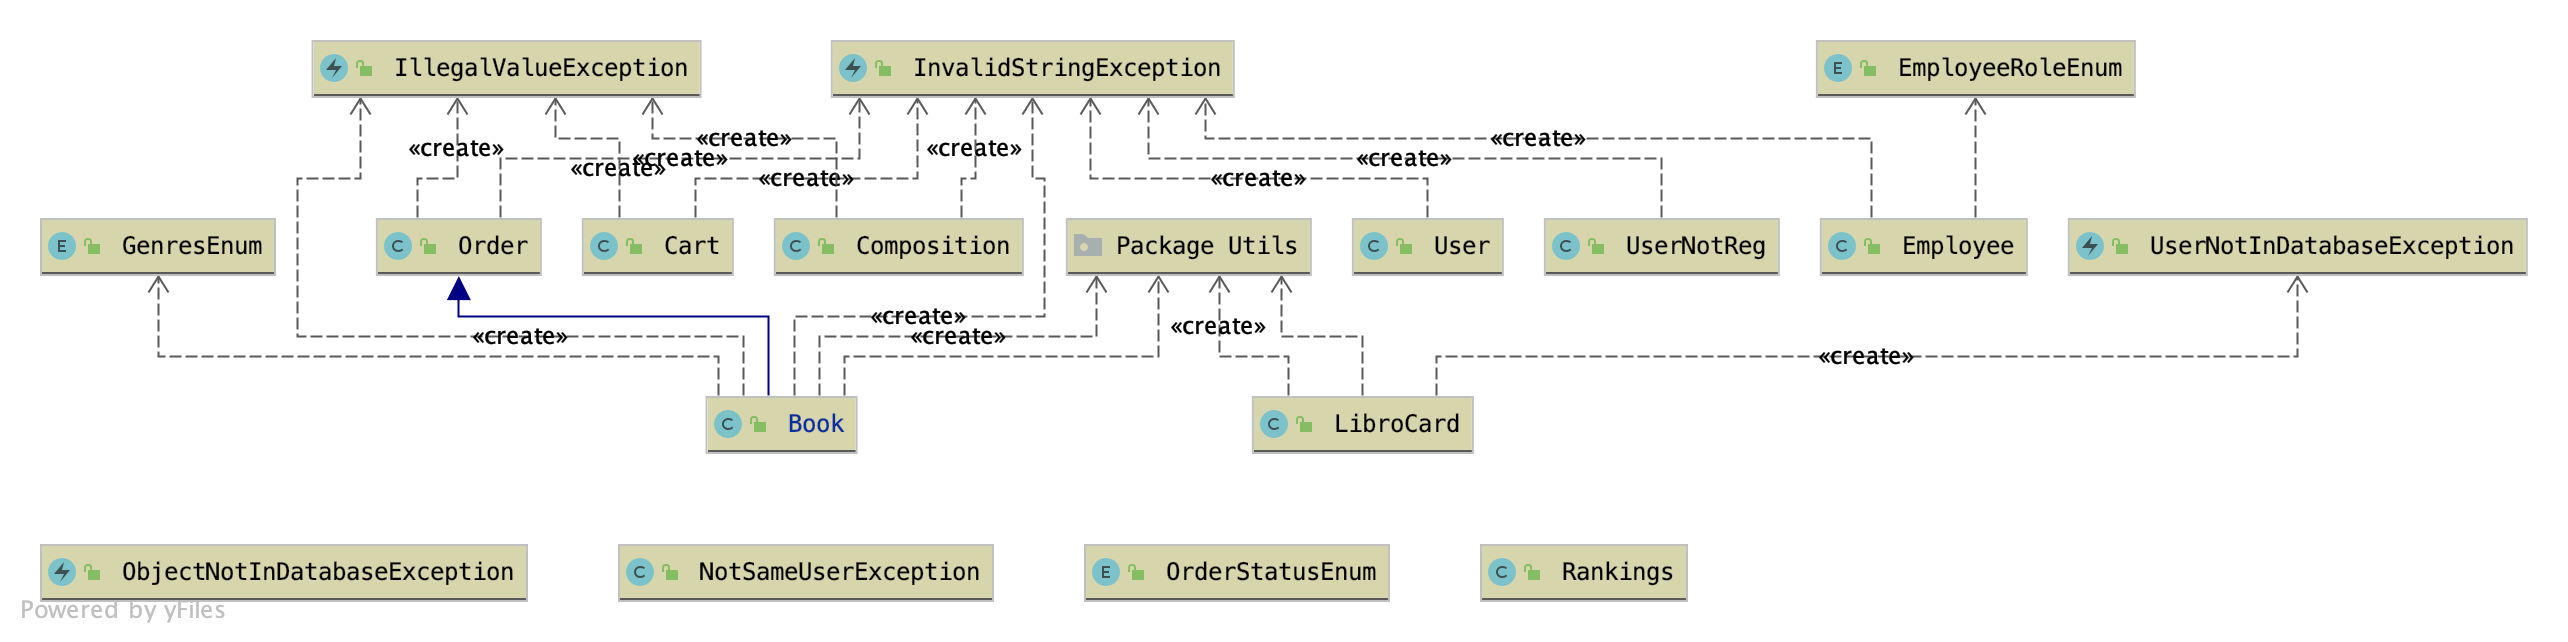
\includegraphics[scale=0.2]{images/ClassDiagrams/ModelClassDiagram.png}
		\caption{Class Diagram per il package Model}
	\end{figure}
	\begin{figure}[h!]
		\centering
		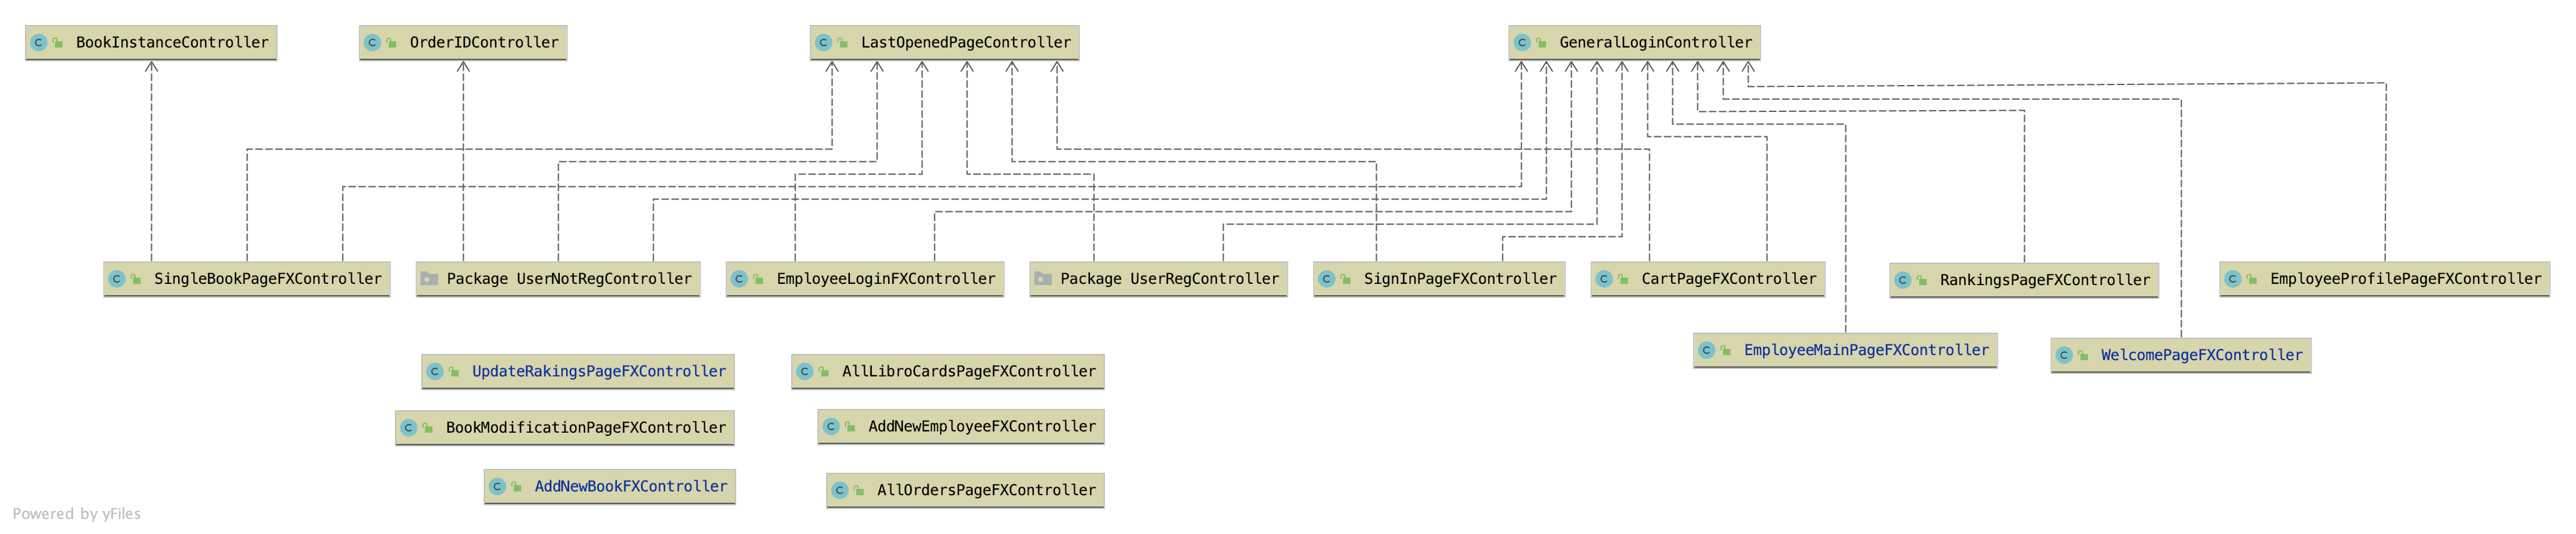
\includegraphics[scale=0.13]{images/ClassDiagrams/ControllerClassDiagram.png}
		\caption{Class Diagram per il package Controller}
	\end{figure}
	\newpage
	\begin{figure}[h!]
		\centering
		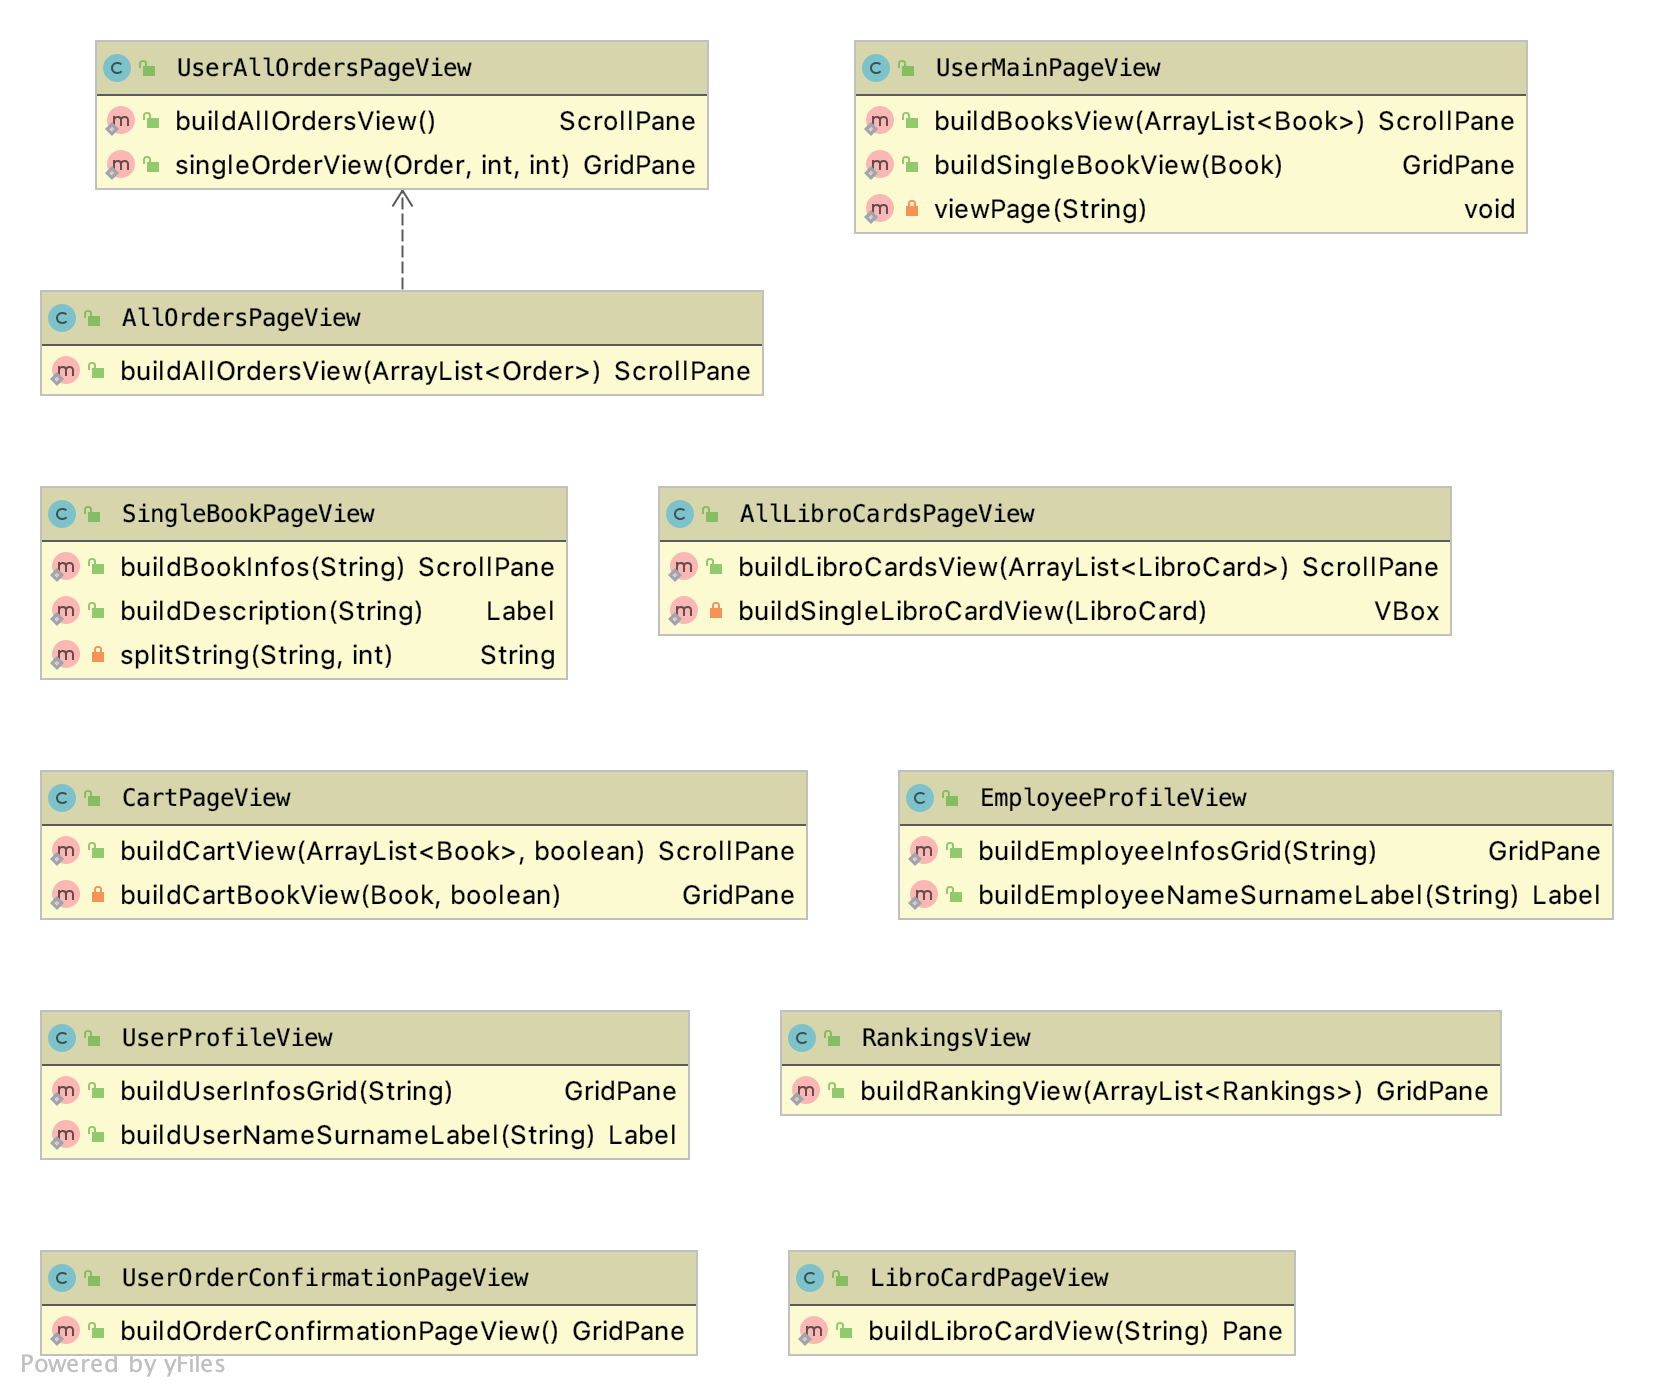
\includegraphics[scale=0.2]{images/ClassDiagrams/ViewClassDiagram.png}
		\caption{Class Diagram per il package View}
	\end{figure}
	\newpage
	\subsection{Sequence Diagrams}
	In questa sezione riportiamo i sequence diagrams, che visualizzano lo scambio di informazioni tra le varie entità nel tempo: il loro scopo è mostrare come un certo comportamento viene realizzato dalla collaborazione delle entità in gioco.
	\begin{figure}[h!]
		\centering
		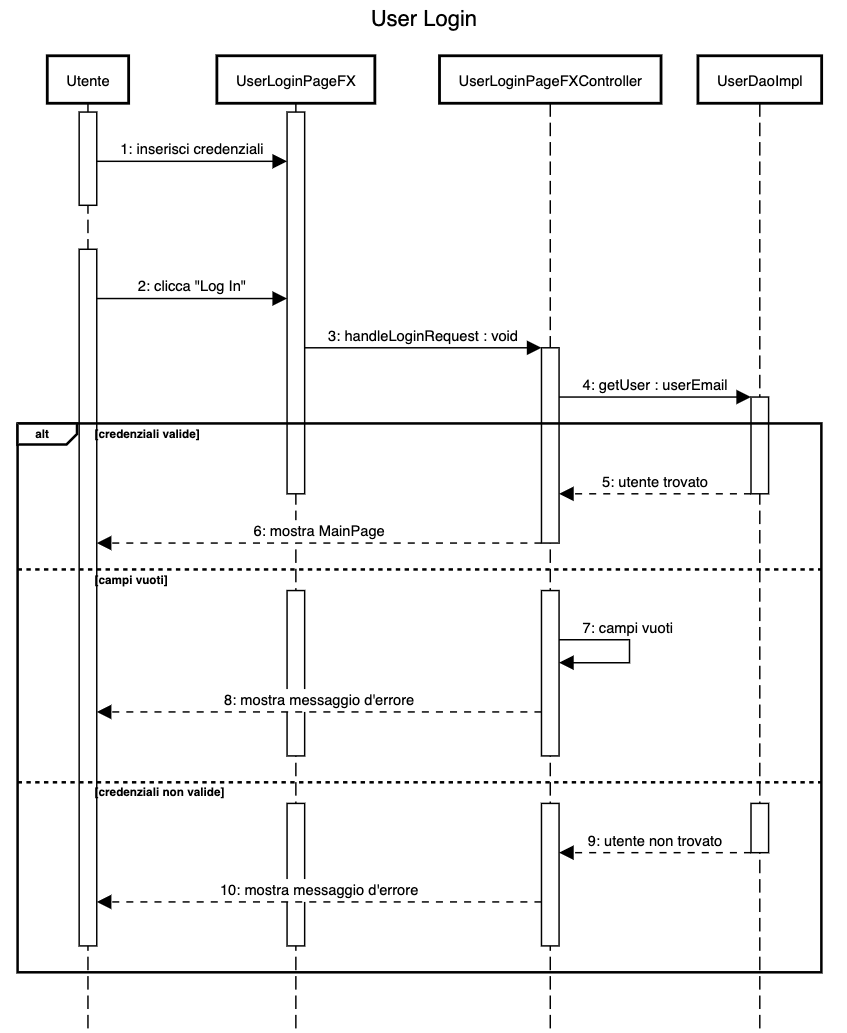
\includegraphics[scale=0.45]{images/SequenceDiagrams/UserLogin.png}
		\caption{Sequence diagram per il \textbf{log in dell'utente}}
	\end{figure}
	\newpage
	\begin{figure}[h!]
		\centering
		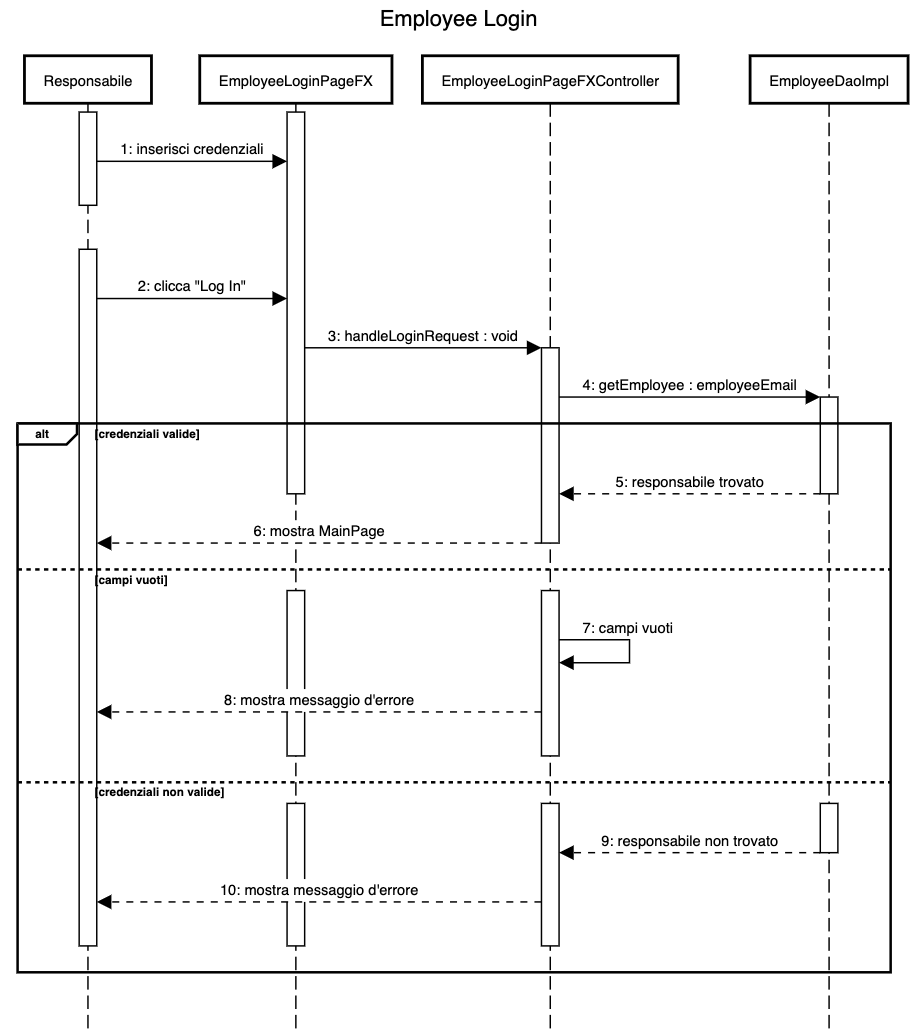
\includegraphics[scale=0.5]{images/SequenceDiagrams/EmployeeLogin.png}
		\caption{Sequence diagram per il \textbf{log in del responsabile}}
	\end{figure}
	\newpage
	\begin{figure}[h!]
		\centering
		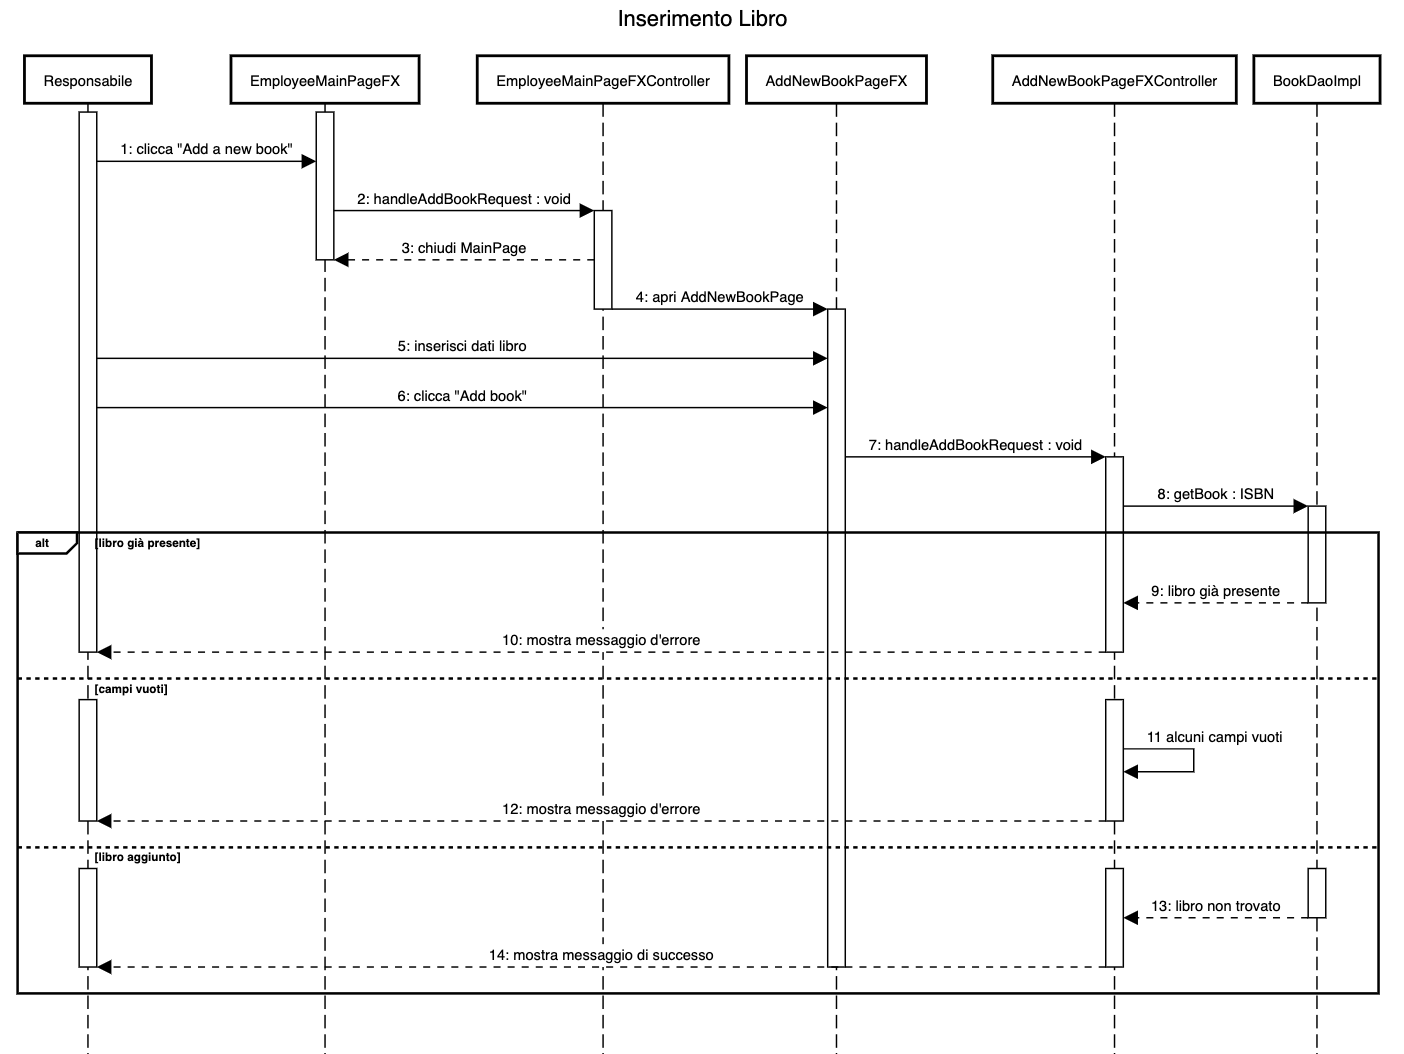
\includegraphics[scale=0.35]{images/SequenceDiagrams/InserimentoLibro.png}
		\caption{Sequence diagram per l'\textbf{inserimento di un nuovo libro}}
	\end{figure}
	\newpage
	\begin{figure}[h!]
		\centering
		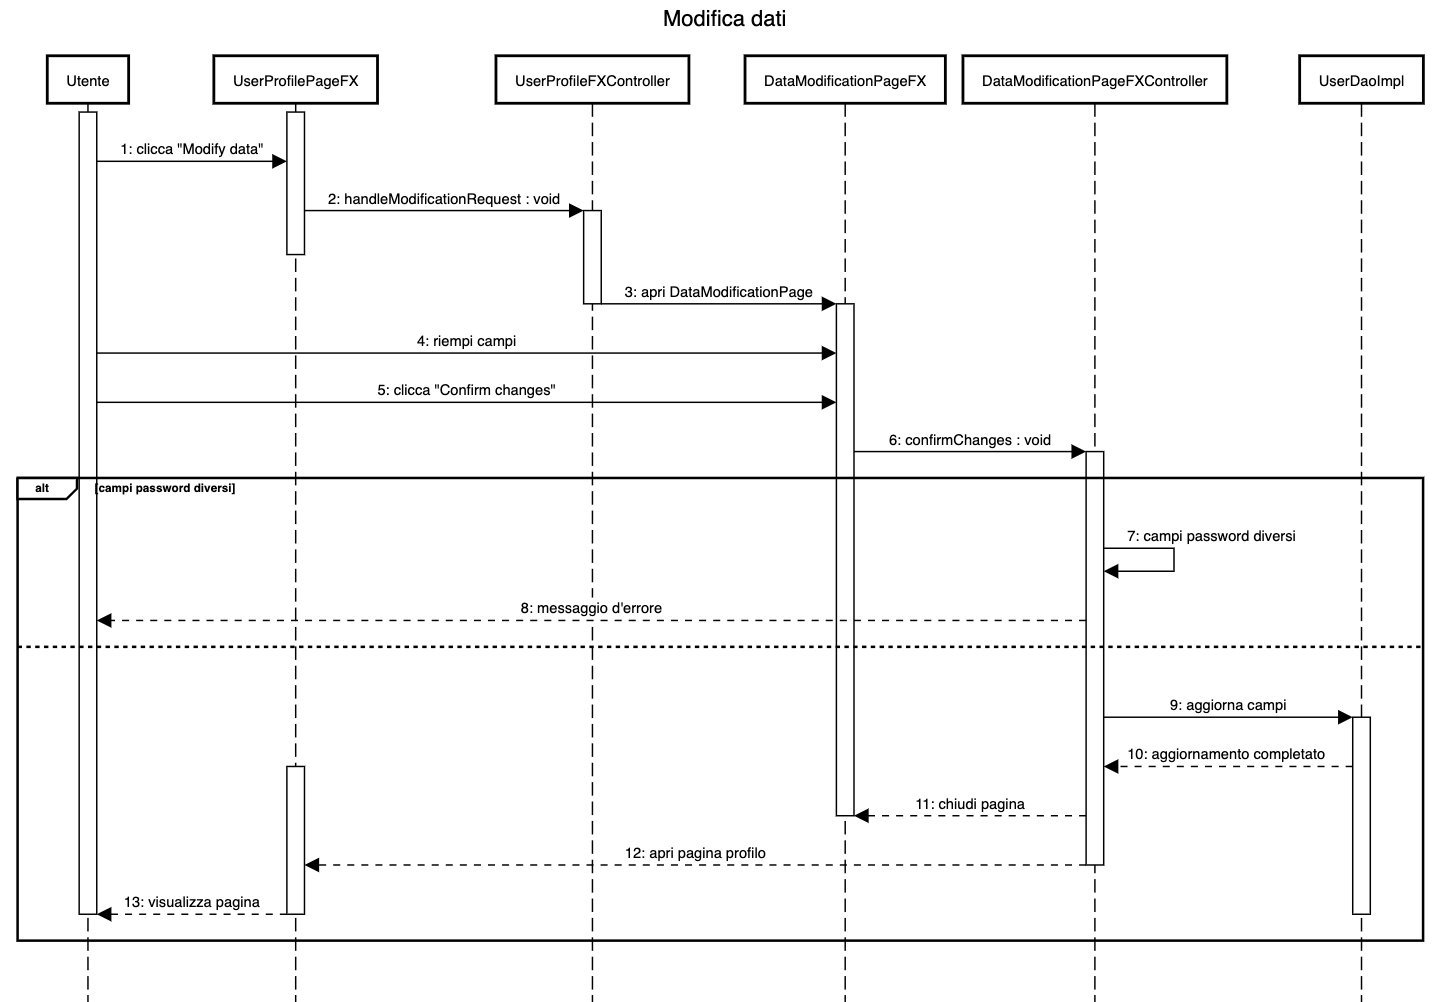
\includegraphics[scale=0.35]{images/SequenceDiagrams/AggiornamentoDati.png}
		\caption{Sequence diagram per la \textbf{modifica dei dati} da parte di un utente}
	\end{figure}
	\newpage
	\begin{figure}[h!]
		\centering
		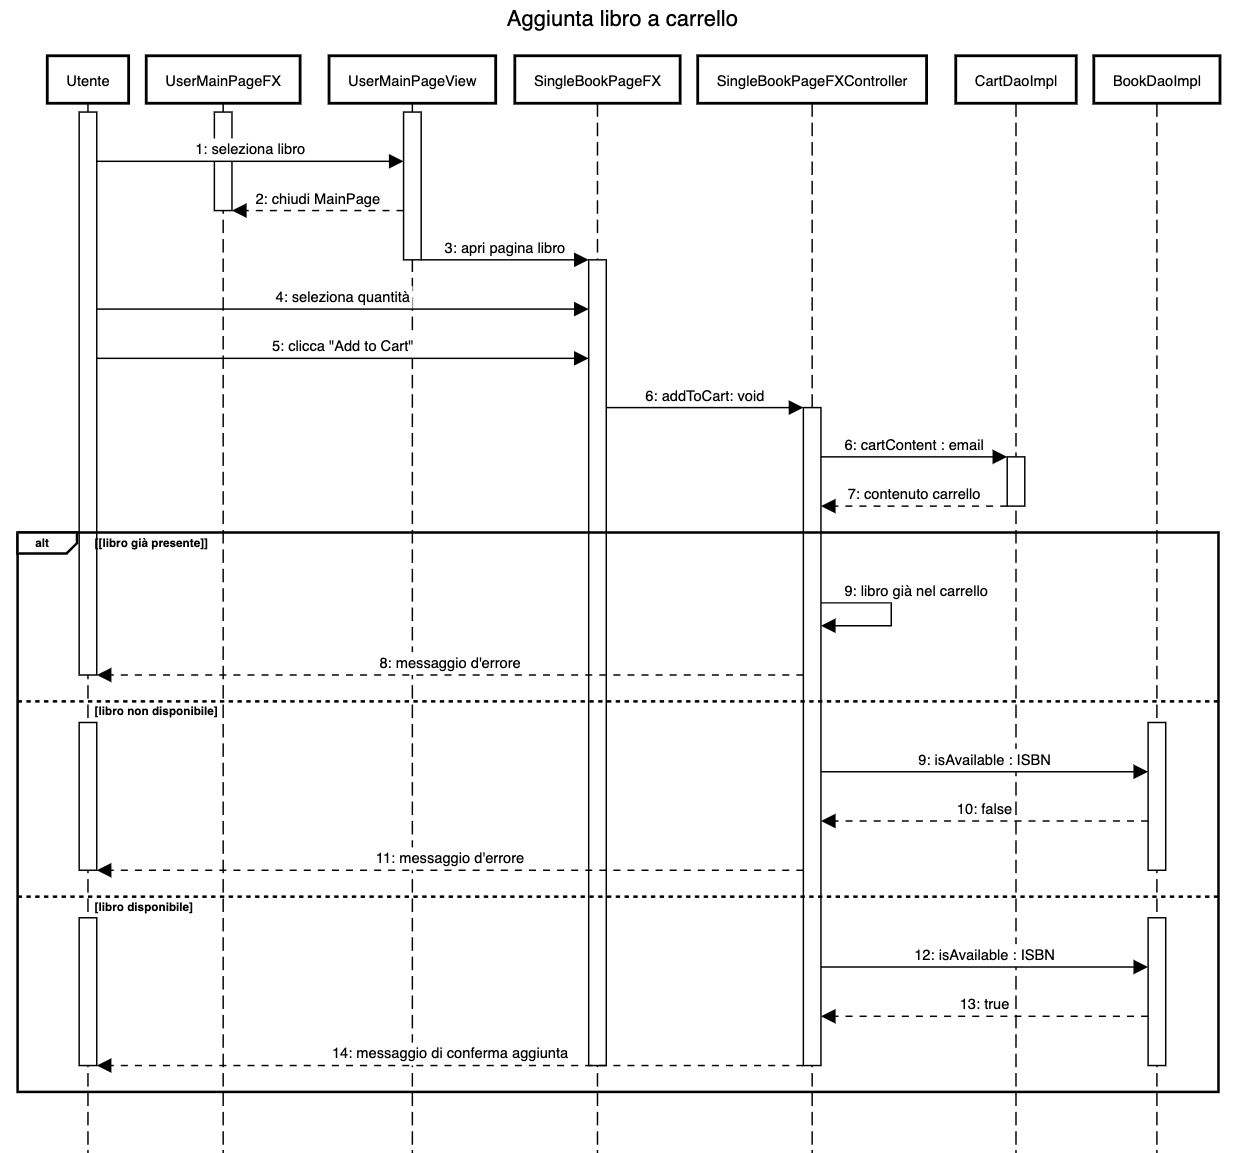
\includegraphics[scale=0.35]{images/SequenceDiagrams/AggiuntaLibro.png}
		\caption{Sequence diagram per la \textbf{aggiunta di un libro} al carrello}
	\end{figure}
	\newpage
	\begin{figure}[h!]
		\centering
		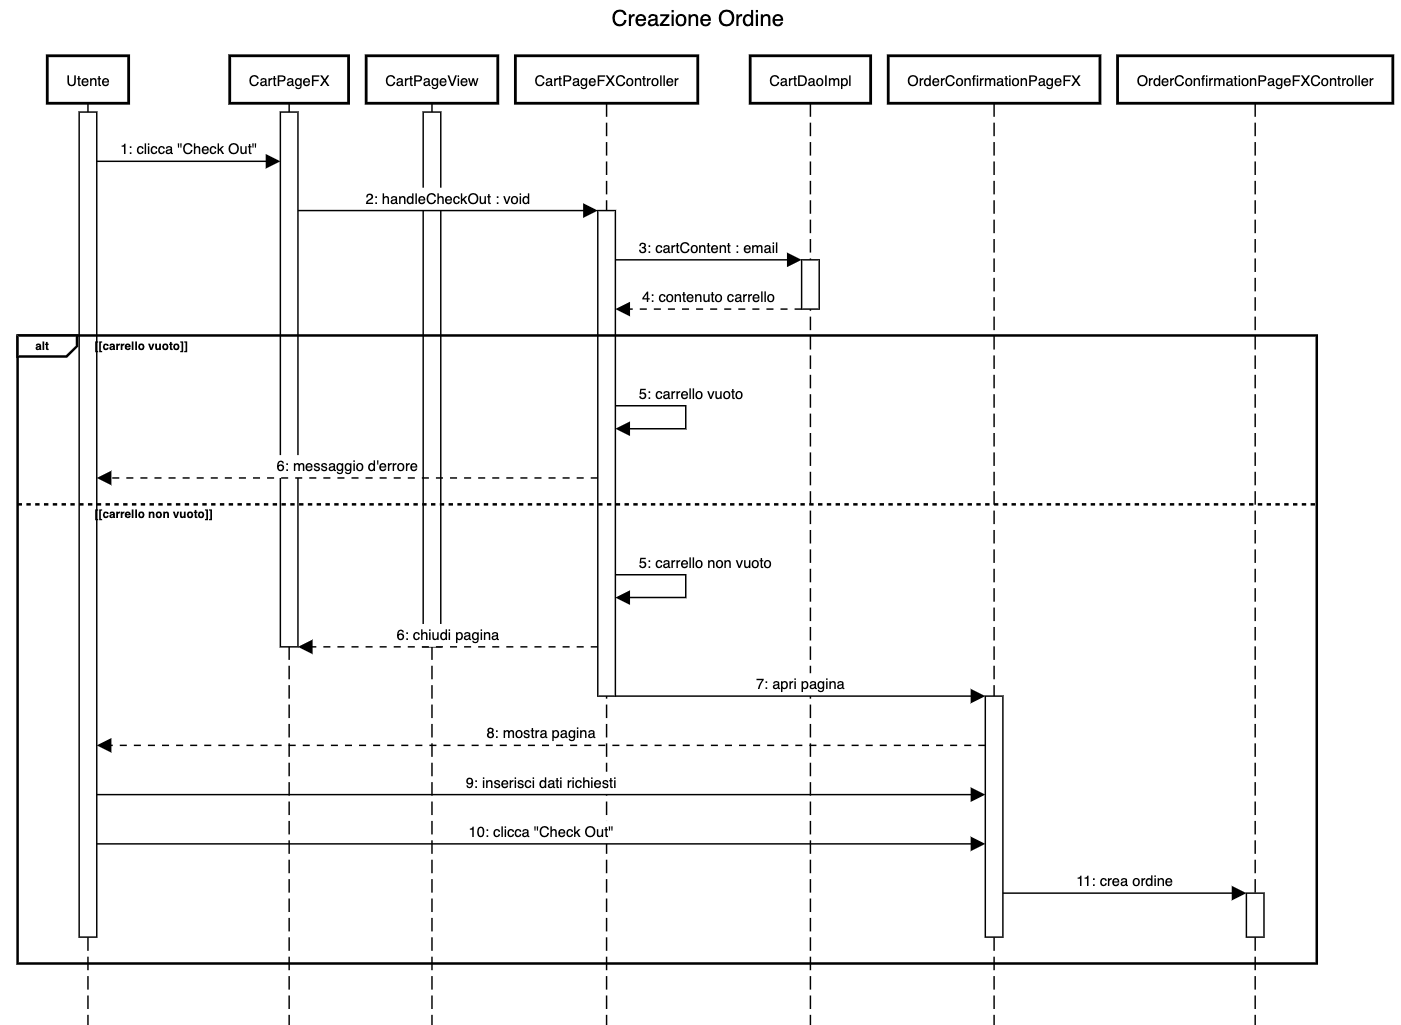
\includegraphics[scale=0.35]{images/SequenceDiagrams/CreazioneOrdine.png}
		\caption{Sequence diagram per la \textbf{creazione di un ordine} da parte di un utente}
	\end{figure}
	\newpage
	\begin{figure}[h!]
		\centering
		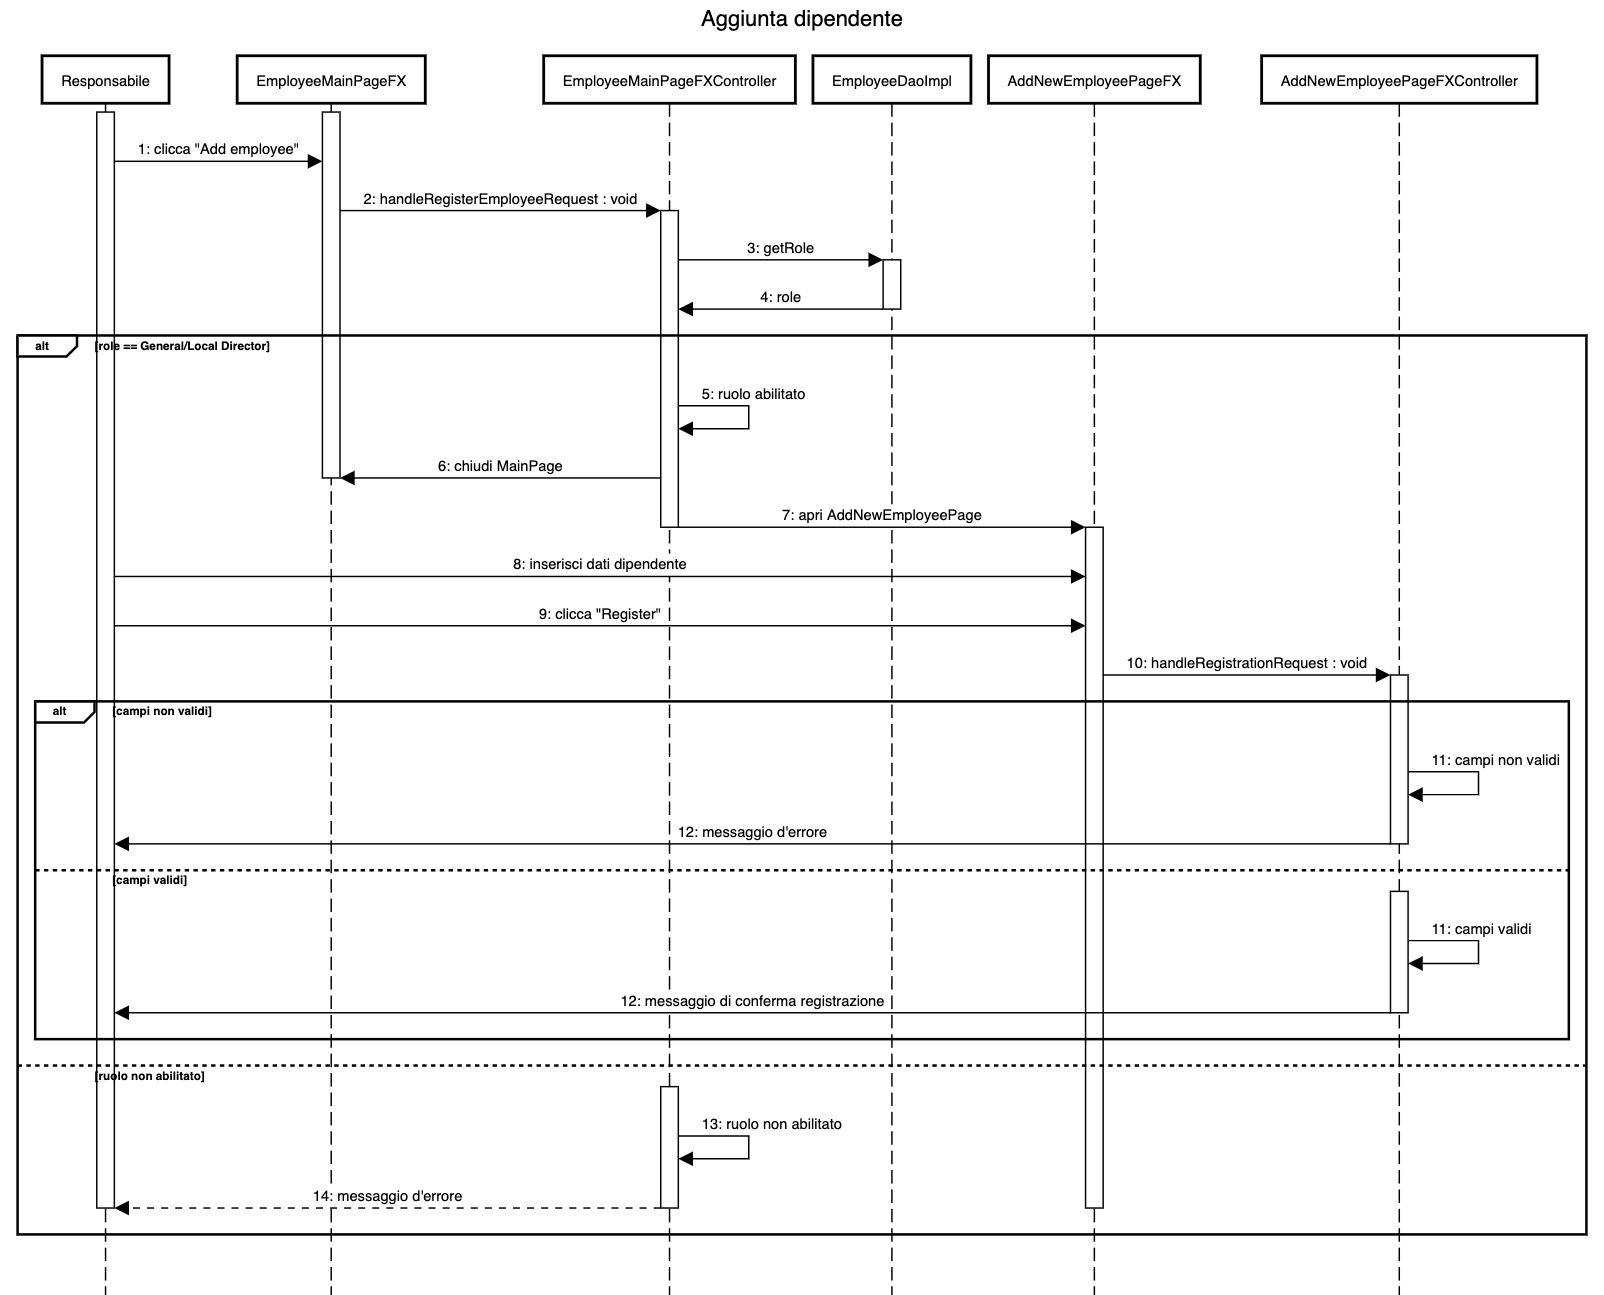
\includegraphics[scale=0.32]{images/SequenceDiagrams/AggiuntaEmployee.png}
		\caption{Sequence diagram per la \textbf{registrazione di un dipendente} da parte di un responsabile}
	\end{figure}
	\newpage
	\section{Scelte progettuali}
	\subsection{Sviluppo} 
	Questo progetto è stato sviluppato principalmente Java, che costituisce un linguaggio estremamente vario e flessibile, e ancora oggi risulta essere molto diffuso nel mercato.\\Per l'interfaccia grafica ho deciso di utilizzare due strumenti: JavaFX, una libreria nativa di Java, e FXML, un linguaggio di mark-up basato su XML. \\JavaFX rappresenta un'alternativa sicuramente più ricca e versatile rispetto a Swing, che è stato invece il tool proposto a lezione: essa permette infatti di realizzare GUI molto più elaborate, grazie alla presenza di animazioni, oggetti geometrici 2D e 3D, grafici, contenuti multimediali, e altro.\\FXML, invece, è stato scelto perché permette di utilizzare un designer di interfacce grafice, Scene Builder, che rende la progettazione sicuramente più semplice e veloce. Inoltre, FXML è particolarmente adatto a interagire con JavaFX, visto che la struttura gerarchica del file rispecchia esattamente la struttura del \textit{scene graph} di JavaFX.\\
	Per stilizzare ulteriormente gli elementi dell'interfaccia grafica si è utilizzato anche CSS, che è completamente supportato sia da JavaFX, sia da FXML.
	\subsection{Database}
	Fin dall'inizio, risultava evidente la necessità di mantenere i dati nel tempo: per questo motivo ho deciso di far uso di un database, sfruttando così anche le conoscenze apprese durante il corso di Database frequentato durante lo sviluppo del progetto.\\
	Dato che la gestione e l'utilizzo del database non rientravano negli obiettivi del progetto, ho scelto di utilizzare SQLite, che costituisce un RDBMS semplice, leggero e open-source.\\
	SQLite è un database engine \textit{"serverless"}: questo significa che i dati vengono memorizzati interamente in locale e non c'è bisogno di stabilire una connessione con un server esterno per lavorare con i dati. In un caso reale, un'applicazione di e-commerce farà chiaramente uso di un'architettura client-server per memorizzare il suo database, ma ricordiamo che il progetto sviluppato rappresenta solo una simulazione di un'applicazione web. \\
	Un altro vantaggio di SQLite è il fatto di essere scritto interamente in C, il che lo rende particolarmente veloce.
	\subsection{MVC Pattern}
	Il funzionamento del progetto è basato sul MVC pattern, che prevede la suddivisione logica delle classi in tre componenti:
	\begin{figure}[h!]
		\centering
		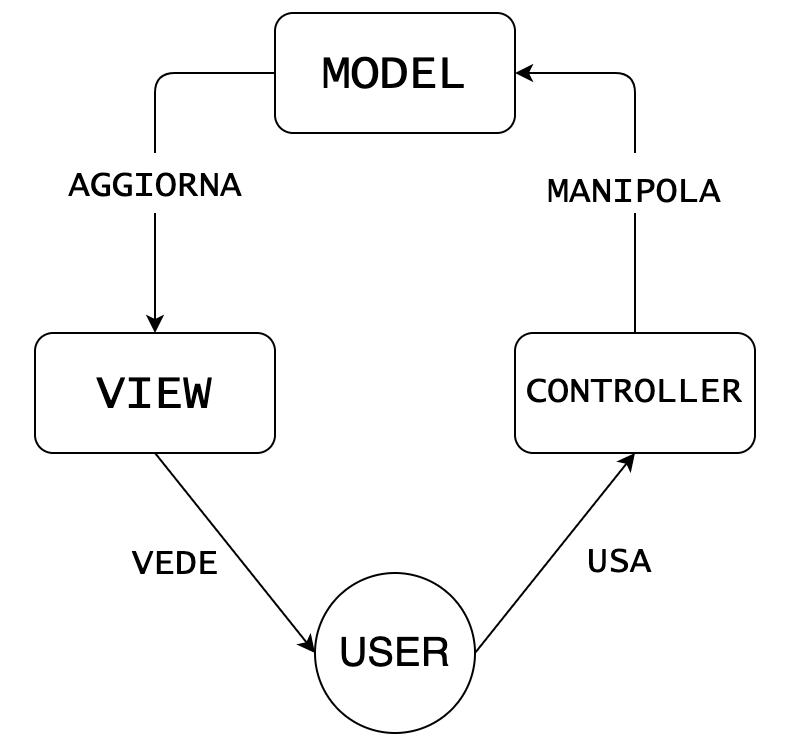
\includegraphics[scale=0.4]{images/MVCPattern.png}
	\end{figure}\\
	Il \textbf{Model} contiene una classe per ogni entità presente nel programma e fornisce i metodi per interagire con esse. Ogni entità contiene dati da memorizzare, infatti all'interno di questo componente troviamo anche le classi che forniscono i metodi per interagire con il database.\\
	Il \textbf{Controller} risponde alle interazioni dell'utente con l'interfaccia grafica attivando determinate procedure ed è il componente che agisce sulle entità del Model.\\
	Il \textbf{View} è la parte di programma che modella l'interfaccia grafica, quindi gestisce il modo in cui i dati vengono presentati all'utente.\\
	I tre componenti del pattern MVC corrispondono concretamente ai tre package principali del programma.
	\subsection{Singleton Pattern}
	Il \textit{Singleton Pattern} è stato utilizzato per limitare l'instanziazione di un oggetto a uno solo. In termini pratici, l'applicazione può essere usata da un solo utente alla volta, e quindi non è possibile essere loggati durante la stessa sessione come due utenti diversi. Nonostante l'applicazione simuli idealmente un sito di e-commerce, quindi un'applicazione web a cui possono accedere più utenti contemporaneamente, nella pratica è stata sviluppata come un'applicazione desktop: di conseguenza il software non è utilizzabile da più persone contemporaneamente, e questo giustifica l'utilizzo di questo design pattern.
	L'implementazione di questo pattern è stata sviluppata nella classe \texttt{GeneralLoginController}: la classe contiene l'attributo \texttt{loginInstance}, inizialmente settato a \texttt{null}, la cui funzione è memorizzare una stringa che identifica univocamente l'utente che ha eseguito il login.\\
	Quando l'utente esegue il logout, il valore della stringa torna ad essere \texttt{null}.\\
	\subsection{Observer Pattern}
	L'\textit{Observer Patter} prevede che un oggetto possa impostare una lista di "ascoltatori" (tecnicamente chiamati \textit{Observers} o \textit{Listeners}) che vengono notificati automaticamente ogni qualvolta lo stato dell'oggetto cambia. 
	Questo pattern è stato utilizzato nell'interfaccia grafica, per ottenere dei cambiamenti dinamici in risposta alle interazioni dell'utente con determinati elementi. \\Più precisamente, è stato impiegato nei seguenti contesti:
	\begin{itemize}
		\item nella \texttt{MainPage} dei clienti (registrati e non), per visualizzare i libri appartenenti a un determinato genere;
		\item nelle \texttt{RankingsPage} dei clienti e dei responsabili, per visualizzare le classifiche relative a un determinato genere;
		\item in \texttt{AllLibroCardsPage}, ovvero la pagina che consente ai responsabili della libreria di controllare le LibroCard degli utenti. In questo caso, l'interfaccia cambiava a seconda che si volesse effettaure la ricerca della LibroCard con l'e-mail dell'utente o con la cardID;
		\item in \texttt{AllOrdersPage}, ovvero la pagina che permette ai responsabili di controllare lo stato degli ordini. In questo caso, l'insieme degli ordini visualizzato cambiava in base allo stato che veniva selezionato.
	\end{itemize}
	\subsection{Data Access Object Pattern}
	Per la gestione del database ho deciso di adottare il \textit{Data Access Object Pattern}, che permette di separare l'insieme delle azioni che l'applicazione ha bisogno di eseguire sul database dal modo in cui esse sono concretamente implementate.\\
	Per ogni classe del \texttt{Model} è stata quindi definita un'interfaccia \texttt{DAO}, contenente la dichiarazione dei metodi tramite cui l'oggetto poteva interagire con il database. Ad ogni interfaccia corrisponde una classe \texttt{DaoImpl} che la implementa, sfruttando l'API di Java per l'interazione con i DBMS, JDBC, e semplici query SQL.
	\section{Validazione}
	Per la validazione dei dati inseriti ho utilizzato ampiamente di oggetti di tipo \texttt{Alert}, messi a disposizione da JavaFX. In questo modo, ho potuto programmare la comparsa di vari tipi di alert a seconda che le condizioni desiderate si verificassero o meno.\\
	Per garantire una corretta esecuzione del programma anche in presenza di errori, ho utilizzato i blocchi \texttt{try-catch}: qualora si verificassero eventi indesiderati che avessero come conseguenza il sollevamento di eccezioni, l'esecuzione dei blocchi \texttt{catch} permettono al programma di segnalare la situazione d'errore senza crashare.
	Per quanto riguarda la GUI non mi è stato possibile testarla automaticamente, ho quindi provveduto ad eseguire un test manuale delle funzionalità.\\
	Mi sono inoltre appoggiata a colleghi ed amici al fine di raccogliere feedback sulle prestazioni del prototipo.
	\section{Conclusioni}
	Obiettivo del progetto non era quello di sviluppare un prodotto finito e completo ma di realizzare un prototipo rispettando le linee guida. Di conseguenza, alcune funzioni sono state realizzate in maniera più semplice rispetto al modo in cui andrebbero implementate nella realtà, e alcuni controlli sono stati resi più "tolleranti".\\Nel complesso, il software sviluppato riesce ad eseguire correttamente tutte le funzioni richieste.
\end{document}